\documentclass[twoside]{book}

% Packages required by doxygen
\usepackage{calc}
\usepackage{doxygen}
\usepackage{graphicx}
\usepackage[utf8]{inputenc}
\usepackage{makeidx}
\usepackage{multicol}
\usepackage{multirow}
\usepackage{textcomp}
\usepackage[table]{xcolor}

% Font selection
\usepackage[T1]{fontenc}
\usepackage{mathptmx}
\usepackage[scaled=.90]{helvet}
\usepackage{courier}
\usepackage{amssymb}
\usepackage{sectsty}
\renewcommand{\familydefault}{\sfdefault}
\allsectionsfont{%
  \fontseries{bc}\selectfont%
  \color{darkgray}%
}
\renewcommand{\DoxyLabelFont}{%
  \fontseries{bc}\selectfont%
  \color{darkgray}%
}

% Page & text layout
\usepackage{geometry}
\geometry{%
  a4paper,%
  top=2.5cm,%
  bottom=2.5cm,%
  left=2.5cm,%
  right=2.5cm%
}
\tolerance=750
\hfuzz=15pt
\hbadness=750
\setlength{\emergencystretch}{15pt}
\setlength{\parindent}{0cm}
\setlength{\parskip}{0.2cm}
\makeatletter
\renewcommand{\paragraph}{%
  \@startsection{paragraph}{4}{0ex}{-1.0ex}{1.0ex}{%
    \normalfont\normalsize\bfseries\SS@parafont%
  }%
}
\renewcommand{\subparagraph}{%
  \@startsection{subparagraph}{5}{0ex}{-1.0ex}{1.0ex}{%
    \normalfont\normalsize\bfseries\SS@subparafont%
  }%
}
\makeatother

% Headers & footers
\usepackage{fancyhdr}
\pagestyle{fancyplain}
\fancyhead[LE]{\fancyplain{}{\bfseries\thepage}}
\fancyhead[CE]{\fancyplain{}{}}
\fancyhead[RE]{\fancyplain{}{\bfseries\leftmark}}
\fancyhead[LO]{\fancyplain{}{\bfseries\rightmark}}
\fancyhead[CO]{\fancyplain{}{}}
\fancyhead[RO]{\fancyplain{}{\bfseries\thepage}}
\fancyfoot[LE]{\fancyplain{}{}}
\fancyfoot[CE]{\fancyplain{}{}}
\fancyfoot[RE]{\fancyplain{}{\bfseries\scriptsize Generated on Thu Apr 9 2015 08\-:19\-:25 for lab4 by Doxygen }}
\fancyfoot[LO]{\fancyplain{}{\bfseries\scriptsize Generated on Thu Apr 9 2015 08\-:19\-:25 for lab4 by Doxygen }}
\fancyfoot[CO]{\fancyplain{}{}}
\fancyfoot[RO]{\fancyplain{}{}}
\renewcommand{\footrulewidth}{0.4pt}
\renewcommand{\chaptermark}[1]{%
  \markboth{#1}{}%
}
\renewcommand{\sectionmark}[1]{%
  \markright{\thesection\ #1}%
}

% Indices & bibliography
\usepackage{natbib}
\usepackage[titles]{tocloft}
\setcounter{tocdepth}{3}
\setcounter{secnumdepth}{5}
\makeindex

% Hyperlinks (required, but should be loaded last)
\usepackage{ifpdf}
\ifpdf
  \usepackage[pdftex,pagebackref=true]{hyperref}
\else
  \usepackage[ps2pdf,pagebackref=true]{hyperref}
\fi
\hypersetup{%
  colorlinks=true,%
  linkcolor=blue,%
  citecolor=blue,%
  unicode%
}

% Custom commands
\newcommand{\clearemptydoublepage}{%
  \newpage{\pagestyle{empty}\cleardoublepage}%
}


%===== C O N T E N T S =====

\begin{document}

% Titlepage & ToC
\hypersetup{pageanchor=false}
\pagenumbering{roman}
\begin{titlepage}
\vspace*{7cm}
\begin{center}%
{\Large lab4 \\[1ex]\large 0.\-0004 }\\
\vspace*{1cm}
{\large Generated by Doxygen 1.8.6}\\
\vspace*{0.5cm}
{\small Thu Apr 9 2015 08:19:25}\\
\end{center}
\end{titlepage}
\clearemptydoublepage
\tableofcontents
\clearemptydoublepage
\pagenumbering{arabic}
\hypersetup{pageanchor=true}

%--- Begin generated contents ---
\chapter{Laboratorium 3}
\label{index}\hypertarget{index}{}\begin{DoxyAuthor}{Author}
Filip Malinowski (Conributor Szymon Furmańczyk) 
\end{DoxyAuthor}
\begin{DoxyDate}{Date}
16.\+04.\+2015 
\end{DoxyDate}
\begin{DoxyVersion}{Version}
0.\+0004
\end{DoxyVersion}
Program sluzacy do uruchamiania algorytmow i badania ich szybkosci dzialania.~\newline
W programie zaimplementowane sa algorytmy\+:~\newline

\begin{DoxyItemize}
\item wczytywanie danej ilosci elementow do stosu~\newline

\item wczytywanie danej ilosci elementow do kolejki~\newline

\item wczytywanie danej ilosci elementow do listy~\newline

\item wczytywanie danej ilosci elementow do listy tablicowej~\newline

\item quicksort tablicy n elementowej
\end{DoxyItemize}

Do wykonania podanych powyzej trzech ostatnich algorytmow zostaly zaimplementowane potrzebne struktury danych (stos, kolejka, lista oraz lista tablicowa).~\newline
~\newline
Ciala klas znajduja sie w folderze ./prj/inc~\newline
Definicje metod znajduja sie w folderze ./prj/src~\newline
Sprawozdanie znajduje sie w folderze ./prj/doc/sprawozdanie~\newline
~\newline
Format wywolania\+:~\newline

\begin{DoxyCode}
./prj/make clean\(\backslash\)n
./prj/make\(\backslash\)n
\end{DoxyCode}
 
\chapter{Hierarchical Index}
\section{Class Hierarchy}
This inheritance list is sorted roughly, but not completely, alphabetically\-:\begin{DoxyCompactList}
\item \contentsline{section}{Benchmark}{\pageref{class_benchmark}}{}
\begin{DoxyCompactList}
\item \contentsline{section}{Algorithm2}{\pageref{class_algorithm2}}{}
\item \contentsline{section}{Algorithm\-Kolejka}{\pageref{class_algorithm_kolejka}}{}
\item \contentsline{section}{Algorithm\-Lista}{\pageref{class_algorithm_lista}}{}
\item \contentsline{section}{Algorithm\-Stos}{\pageref{class_algorithm_stos}}{}
\item \contentsline{section}{Mnozenie}{\pageref{class_mnozenie}}{}
\end{DoxyCompactList}
\item \contentsline{section}{Kolejka}{\pageref{class_kolejka}}{}
\item \contentsline{section}{Lista\-:\-:Komorka}{\pageref{struct_lista_1_1_komorka}}{}
\item \contentsline{section}{Lista}{\pageref{class_lista}}{}
\item \contentsline{section}{Stos}{\pageref{class_stos}}{}
\item \contentsline{section}{Tab\-Lista}{\pageref{class_tab_lista}}{}
\end{DoxyCompactList}

\chapter{Class Index}
\section{Class List}
Here are the classes, structs, unions and interfaces with brief descriptions\-:\begin{DoxyCompactList}
\item\contentsline{section}{\hyperlink{class_algorithm2}{Algorithm2} \\*Klasa \hyperlink{class_algorithm2}{Algorithm2} modelujaca algorytm wczytywania do listy tablicowej. Obiekt tego typu reprezentuje algorytm wykonujacy wykonujacy wczytywanie zadanej ilosci elementow do listy tablicowej }{\pageref{class_algorithm2}}{}
\item\contentsline{section}{\hyperlink{class_algorithm_kolejka}{Algorithm\-Kolejka} \\*Klasa \hyperlink{class_algorithm_kolejka}{Algorithm\-Kolejka} modelujaca algorytm wczytywania do kolejki. Obiekt tego typu reprezentuje algorytm wykonujacy wykonujacy wczytywanie zadanej ilosci elementow do kolejki }{\pageref{class_algorithm_kolejka}}{}
\item\contentsline{section}{\hyperlink{class_algorithm_lista}{Algorithm\-Lista} \\*Klasa \hyperlink{class_algorithm_lista}{Algorithm\-Lista} modelujaca algorytm wczytywania do kolejki. Obiekt tego typu reprezentuje algorytm wykonujacy wykonujacy wczytywanie zadanej ilosci elementow do listy }{\pageref{class_algorithm_lista}}{}
\item\contentsline{section}{\hyperlink{class_algorithm_stos}{Algorithm\-Stos} \\*Klasa \hyperlink{class_algorithm_stos}{Algorithm\-Stos} modelujaca algorytm wczytywania do stosu. Obiekt tego typu reprezentuje algorytm wykonujacy wykonujacy wczytywanie zadanej ilosci elementow do stosu }{\pageref{class_algorithm_stos}}{}
\item\contentsline{section}{\hyperlink{class_benchmark}{Benchmark} \\*Klasa \hyperlink{class_benchmark}{Benchmark} modelujaca program benchmarkujacy. Obiekt tego typu reprezentuje program sprawdzajacy szybkosc wykonywania algorytmow }{\pageref{class_benchmark}}{}
\item\contentsline{section}{\hyperlink{class_kolejka}{Kolejka} \\*Klasa \hyperlink{class_kolejka}{Kolejka} modelujaca strukture danych typu kolejka. Obiekt tego typu reprezentuje strukture danych typu kolejka wraz z operacjami mozliwymi do wykonania na tej strukturze }{\pageref{class_kolejka}}{}
\item\contentsline{section}{\hyperlink{struct_lista_1_1_komorka}{Lista\-::\-Komorka} \\*Struktura \hyperlink{struct_lista_1_1_komorka}{Komorka}. Obiekt tego typu reprezentuje pojedyncza komorke wraz ze wskaznikiem na nastepna komorke listy }{\pageref{struct_lista_1_1_komorka}}{}
\item\contentsline{section}{\hyperlink{class_lista}{Lista} \\*Klasa \hyperlink{class_lista}{Lista} modelujaca strukture danych typu lista. Obiekt tego typu reprezentuje strukture danych typu lista wraz z operacjami mozliwymi do wykonania na tej strukturze }{\pageref{class_lista}}{}
\item\contentsline{section}{\hyperlink{class_mnozenie}{Mnozenie} \\*Klasa \hyperlink{class_mnozenie}{Mnozenie} modelujaca algorytm mnozenia. Obiekt tego typu reprezentuje algorytm wykonujacy dzialanie mnozenia kazdego elementu tablicy tab przez 2 }{\pageref{class_mnozenie}}{}
\item\contentsline{section}{\hyperlink{class_stos}{Stos} \\*Klasa \hyperlink{class_stos}{Stos} modelujaca strukture danych typu stos. Obiekt tego typu reprezentuje strukture danych typu stos wraz z operacjami mozliwymi do wykonania na tej strukturze }{\pageref{class_stos}}{}
\item\contentsline{section}{\hyperlink{class_tab_lista}{Tab\-Lista} \\*Klasa \hyperlink{class_tab_lista}{Tab\-Lista} modelujaca strukture danych typu lista. Obiekt tego typu reprezentuje strukture danych typu lista zaimplementowana na tablicy dynamicznej. Obiekt zawiera rowniez podstowe metody listy }{\pageref{class_tab_lista}}{}
\end{DoxyCompactList}

\chapter{File Index}
\section{File List}
Here is a list of all files with brief descriptions\-:\begin{DoxyCompactList}
\item\contentsline{section}{\hyperlink{algorithm1_8cpp}{algorithm1.\-cpp} }{\pageref{algorithm1_8cpp}}{}
\item\contentsline{section}{\hyperlink{algorithm1_8hh}{algorithm1.\-hh} }{\pageref{algorithm1_8hh}}{}
\item\contentsline{section}{\hyperlink{algorithm2_8cpp}{algorithm2.\-cpp} }{\pageref{algorithm2_8cpp}}{}
\item\contentsline{section}{\hyperlink{algorithm2_8hh}{algorithm2.\-hh} }{\pageref{algorithm2_8hh}}{}
\item\contentsline{section}{\hyperlink{algorithm__kolejka_8cpp}{algorithm\-\_\-kolejka.\-cpp} }{\pageref{algorithm__kolejka_8cpp}}{}
\item\contentsline{section}{\hyperlink{algorithm__kolejka_8hh}{algorithm\-\_\-kolejka.\-hh} }{\pageref{algorithm__kolejka_8hh}}{}
\item\contentsline{section}{\hyperlink{algorithm__lista_8cpp}{algorithm\-\_\-lista.\-cpp} }{\pageref{algorithm__lista_8cpp}}{}
\item\contentsline{section}{\hyperlink{algorithm__lista_8hh}{algorithm\-\_\-lista.\-hh} }{\pageref{algorithm__lista_8hh}}{}
\item\contentsline{section}{\hyperlink{algorithm__stos_8cpp}{algorithm\-\_\-stos.\-cpp} }{\pageref{algorithm__stos_8cpp}}{}
\item\contentsline{section}{\hyperlink{algorithm__stos_8hh}{algorithm\-\_\-stos.\-hh} }{\pageref{algorithm__stos_8hh}}{}
\item\contentsline{section}{\hyperlink{benchmark_8cpp}{benchmark.\-cpp} }{\pageref{benchmark_8cpp}}{}
\item\contentsline{section}{\hyperlink{benchmark_8hh}{benchmark.\-hh} }{\pageref{benchmark_8hh}}{}
\item\contentsline{section}{\hyperlink{generate_8cpp}{generate.\-cpp} }{\pageref{generate_8cpp}}{}
\item\contentsline{section}{\hyperlink{kolejka_8cpp}{kolejka.\-cpp} }{\pageref{kolejka_8cpp}}{}
\item\contentsline{section}{\hyperlink{kolejka_8hh}{kolejka.\-hh} }{\pageref{kolejka_8hh}}{}
\item\contentsline{section}{\hyperlink{lista_8cpp}{lista.\-cpp} }{\pageref{lista_8cpp}}{}
\item\contentsline{section}{\hyperlink{lista_8hh}{lista.\-hh} }{\pageref{lista_8hh}}{}
\item\contentsline{section}{\hyperlink{main_8cpp}{main.\-cpp} }{\pageref{main_8cpp}}{}
\item\contentsline{section}{\hyperlink{stos_8cpp}{stos.\-cpp} }{\pageref{stos_8cpp}}{}
\item\contentsline{section}{\hyperlink{stos_8hh}{stos.\-hh} }{\pageref{stos_8hh}}{}
\item\contentsline{section}{\hyperlink{tab__lista_8cpp}{tab\-\_\-lista.\-cpp} }{\pageref{tab__lista_8cpp}}{}
\item\contentsline{section}{\hyperlink{tab__lista_8hh}{tab\-\_\-lista.\-hh} }{\pageref{tab__lista_8hh}}{}
\end{DoxyCompactList}

\chapter{Class Documentation}
\hypertarget{class_algorithm2}{}\section{Algorithm2 Class Reference}
\label{class_algorithm2}\index{Algorithm2@{Algorithm2}}


Klasa \hyperlink{class_algorithm2}{Algorithm2} modelujaca algorytm wczytywania do listy tablicowej. Obiekt tego typu reprezentuje algorytm wykonujacy wykonujacy wczytywanie zadanej ilosci elementow do listy tablicowej.  




{\ttfamily \#include $<$algorithm2.\+hh$>$}



Inheritance diagram for Algorithm2\+:\nopagebreak
\begin{figure}[H]
\begin{center}
\leavevmode
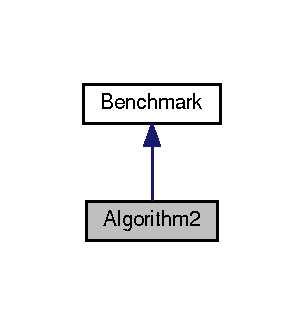
\includegraphics[width=146pt]{class_algorithm2__inherit__graph}
\end{center}
\end{figure}


Collaboration diagram for Algorithm2\+:\nopagebreak
\begin{figure}[H]
\begin{center}
\leavevmode
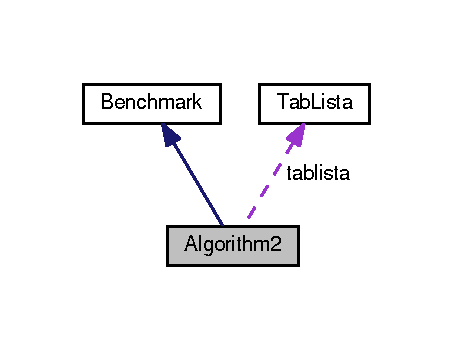
\includegraphics[width=217pt]{class_algorithm2__coll__graph}
\end{center}
\end{figure}
\subsection*{Public Member Functions}
\begin{DoxyCompactItemize}
\item 
\hyperlink{class_algorithm2_ad77a51433815456eca8139444e78b49b}{Algorithm2} ()
\begin{DoxyCompactList}\small\item\em Konstruktor obiektu \hyperlink{class_algorithm2}{Algorithm2}. \end{DoxyCompactList}\item 
\hyperlink{class_algorithm2_ac5cc064a2727d2c1a2b32d335cd73f8d}{Algorithm2} (int \+\_\+tab\mbox{[}$\,$\mbox{]})
\begin{DoxyCompactList}\small\item\em Konstruktor parametryczny obiektu \hyperlink{class_algorithm2}{Algorithm2}. \end{DoxyCompactList}\item 
\hyperlink{class_algorithm2_ab2c630f56f5d2e90f62a13fdaf0cd954}{$\sim$\+Algorithm2} ()
\begin{DoxyCompactList}\small\item\em Destruktor obiektu \hyperlink{class_algorithm2}{Algorithm2}. \end{DoxyCompactList}\item 
virtual void \hyperlink{class_algorithm2_a6eb066d5e51f2187e717454751bc2934}{test\+Algorithm} (\hyperlink{class_benchmark}{Benchmark} $\ast$\+\_\+algorithm)
\begin{DoxyCompactList}\small\item\em Metoda testowania algorytmu. Metoda sluzy do testowania szybkosci dzialania algorytmu. W klasie \hyperlink{class_algorithm2}{Algorithm2} nie ma konkretnego dzialania. \end{DoxyCompactList}\item 
virtual void \hyperlink{class_algorithm2_a409e58d5fb0b6d2407cc986cf163703b}{run\+Algorithm} (int \+\_\+border)
\begin{DoxyCompactList}\small\item\em Metoda uruchamiania algorytmu. Metoda sluzy to wykonywania danego algorytmu. Wczytuje elementy do kolejki. \end{DoxyCompactList}\item 
virtual void \hyperlink{class_algorithm2_a103c600d6f7a33872672e4b26d89475f}{run\+Algorithm\+Szybkie\+Sortowanie} ()
\begin{DoxyCompactList}\small\item\em Metoda uruchamiania algorytmu szybkiego sortowania. Metoda sluzy to wykonywania danego algorytmu. Sortuje tablicę. \end{DoxyCompactList}\end{DoxyCompactItemize}
\subsection*{Private Attributes}
\begin{DoxyCompactItemize}
\item 
int \hyperlink{class_algorithm2_a4a2c5e1211591fb0ad00d64ca783bf56}{tab} \mbox{[}\hyperlink{benchmark_8hh_a70ed59adcb4159ac551058053e649640}{S\+I\+Z\+E}\mbox{]}
\begin{DoxyCompactList}\small\item\em Tablica elementow z danymi wejsciowymi. \end{DoxyCompactList}\item 
\hyperlink{class_tab_lista}{Tab\+Lista} \hyperlink{class_algorithm2_af58d491bdb13e788c40754617f3b13df}{tablista}
\begin{DoxyCompactList}\small\item\em Zmienna przechowujaca liste tablicowa. \end{DoxyCompactList}\end{DoxyCompactItemize}


\subsection{Detailed Description}


Definition at line 9 of file algorithm2.\+hh.



\subsection{Constructor \& Destructor Documentation}
\hypertarget{class_algorithm2_ad77a51433815456eca8139444e78b49b}{}\index{Algorithm2@{Algorithm2}!Algorithm2@{Algorithm2}}
\index{Algorithm2@{Algorithm2}!Algorithm2@{Algorithm2}}
\subsubsection[{Algorithm2}]{\setlength{\rightskip}{0pt plus 5cm}Algorithm2\+::\+Algorithm2 (
\begin{DoxyParamCaption}
{}
\end{DoxyParamCaption}
)\hspace{0.3cm}{\ttfamily [inline]}}\label{class_algorithm2_ad77a51433815456eca8139444e78b49b}


Definition at line 24 of file algorithm2.\+hh.

\hypertarget{class_algorithm2_ac5cc064a2727d2c1a2b32d335cd73f8d}{}\index{Algorithm2@{Algorithm2}!Algorithm2@{Algorithm2}}
\index{Algorithm2@{Algorithm2}!Algorithm2@{Algorithm2}}
\subsubsection[{Algorithm2}]{\setlength{\rightskip}{0pt plus 5cm}Algorithm2\+::\+Algorithm2 (
\begin{DoxyParamCaption}
\item[{int}]{\+\_\+tab\mbox{[}$\,$\mbox{]}}
\end{DoxyParamCaption}
)\hspace{0.3cm}{\ttfamily [inline]}}\label{class_algorithm2_ac5cc064a2727d2c1a2b32d335cd73f8d}

\begin{DoxyParams}[1]{Parameters}
\mbox{\tt in}  & {\em \+\_\+tab} & -\/ tablica przechowujaca dane wejsciowe. \\
\hline
\end{DoxyParams}


Definition at line 30 of file algorithm2.\+hh.

\hypertarget{class_algorithm2_ab2c630f56f5d2e90f62a13fdaf0cd954}{}\index{Algorithm2@{Algorithm2}!````~Algorithm2@{$\sim$\+Algorithm2}}
\index{````~Algorithm2@{$\sim$\+Algorithm2}!Algorithm2@{Algorithm2}}
\subsubsection[{$\sim$\+Algorithm2}]{\setlength{\rightskip}{0pt plus 5cm}Algorithm2\+::$\sim$\+Algorithm2 (
\begin{DoxyParamCaption}
{}
\end{DoxyParamCaption}
)\hspace{0.3cm}{\ttfamily [inline]}}\label{class_algorithm2_ab2c630f56f5d2e90f62a13fdaf0cd954}


Definition at line 35 of file algorithm2.\+hh.



\subsection{Member Function Documentation}
\hypertarget{class_algorithm2_a409e58d5fb0b6d2407cc986cf163703b}{}\index{Algorithm2@{Algorithm2}!run\+Algorithm@{run\+Algorithm}}
\index{run\+Algorithm@{run\+Algorithm}!Algorithm2@{Algorithm2}}
\subsubsection[{run\+Algorithm}]{\setlength{\rightskip}{0pt plus 5cm}void Algorithm2\+::run\+Algorithm (
\begin{DoxyParamCaption}
\item[{int}]{\+\_\+border}
\end{DoxyParamCaption}
)\hspace{0.3cm}{\ttfamily [virtual]}}\label{class_algorithm2_a409e58d5fb0b6d2407cc986cf163703b}

\begin{DoxyParams}[1]{Parameters}
\mbox{\tt in}  & {\em \+\_\+border} & -\/ ilosc elementow dla ktorych algorytm ma wykonac swoje dzialanie. \\
\hline
\end{DoxyParams}


Reimplemented from \hyperlink{class_benchmark_a6363894c058e8bfe146de09d7126b29c}{Benchmark}.



Definition at line 8 of file algorithm2.\+cpp.



Here is the call graph for this function\+:\nopagebreak
\begin{figure}[H]
\begin{center}
\leavevmode
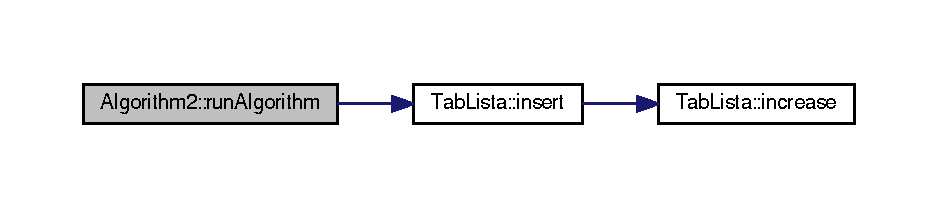
\includegraphics[width=350pt]{class_algorithm2_a409e58d5fb0b6d2407cc986cf163703b_cgraph}
\end{center}
\end{figure}


\hypertarget{class_algorithm2_a103c600d6f7a33872672e4b26d89475f}{}\index{Algorithm2@{Algorithm2}!run\+Algorithm\+Szybkie\+Sortowanie@{run\+Algorithm\+Szybkie\+Sortowanie}}
\index{run\+Algorithm\+Szybkie\+Sortowanie@{run\+Algorithm\+Szybkie\+Sortowanie}!Algorithm2@{Algorithm2}}
\subsubsection[{run\+Algorithm\+Szybkie\+Sortowanie}]{\setlength{\rightskip}{0pt plus 5cm}void Algorithm2\+::run\+Algorithm\+Szybkie\+Sortowanie (
\begin{DoxyParamCaption}
{}
\end{DoxyParamCaption}
)\hspace{0.3cm}{\ttfamily [virtual]}}\label{class_algorithm2_a103c600d6f7a33872672e4b26d89475f}


Reimplemented from \hyperlink{class_benchmark_a05a8e8b9b80949f51c2ccc47e08dedbb}{Benchmark}.



Definition at line 17 of file algorithm2.\+cpp.



Here is the call graph for this function\+:\nopagebreak
\begin{figure}[H]
\begin{center}
\leavevmode
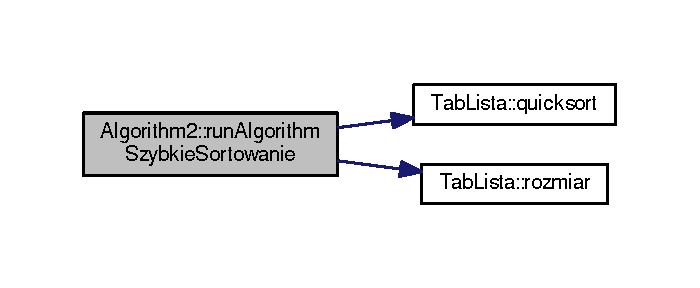
\includegraphics[width=336pt]{class_algorithm2_a103c600d6f7a33872672e4b26d89475f_cgraph}
\end{center}
\end{figure}


\hypertarget{class_algorithm2_a6eb066d5e51f2187e717454751bc2934}{}\index{Algorithm2@{Algorithm2}!test\+Algorithm@{test\+Algorithm}}
\index{test\+Algorithm@{test\+Algorithm}!Algorithm2@{Algorithm2}}
\subsubsection[{test\+Algorithm}]{\setlength{\rightskip}{0pt plus 5cm}virtual void Algorithm2\+::test\+Algorithm (
\begin{DoxyParamCaption}
\item[{{\bf Benchmark} $\ast$}]{\+\_\+algorithm}
\end{DoxyParamCaption}
)\hspace{0.3cm}{\ttfamily [inline]}, {\ttfamily [virtual]}}\label{class_algorithm2_a6eb066d5e51f2187e717454751bc2934}

\begin{DoxyParams}[1]{Parameters}
\mbox{\tt in}  & {\em \+\_\+algorithm} & -\/ testowany algorytm. \\
\hline
\end{DoxyParams}


Definition at line 43 of file algorithm2.\+hh.



\subsection{Member Data Documentation}
\hypertarget{class_algorithm2_a4a2c5e1211591fb0ad00d64ca783bf56}{}\index{Algorithm2@{Algorithm2}!tab@{tab}}
\index{tab@{tab}!Algorithm2@{Algorithm2}}
\subsubsection[{tab}]{\setlength{\rightskip}{0pt plus 5cm}int Algorithm2\+::tab\mbox{[}{\bf S\+I\+Z\+E}\mbox{]}\hspace{0.3cm}{\ttfamily [private]}}\label{class_algorithm2_a4a2c5e1211591fb0ad00d64ca783bf56}


Definition at line 14 of file algorithm2.\+hh.

\hypertarget{class_algorithm2_af58d491bdb13e788c40754617f3b13df}{}\index{Algorithm2@{Algorithm2}!tablista@{tablista}}
\index{tablista@{tablista}!Algorithm2@{Algorithm2}}
\subsubsection[{tablista}]{\setlength{\rightskip}{0pt plus 5cm}{\bf Tab\+Lista} Algorithm2\+::tablista\hspace{0.3cm}{\ttfamily [private]}}\label{class_algorithm2_af58d491bdb13e788c40754617f3b13df}


Definition at line 18 of file algorithm2.\+hh.



The documentation for this class was generated from the following files\+:\begin{DoxyCompactItemize}
\item 
\hyperlink{algorithm2_8hh}{algorithm2.\+hh}\item 
\hyperlink{algorithm2_8cpp}{algorithm2.\+cpp}\end{DoxyCompactItemize}

\hypertarget{class_algorithm_kolejka}{}\section{Algorithm\+Kolejka Class Reference}
\label{class_algorithm_kolejka}\index{Algorithm\+Kolejka@{Algorithm\+Kolejka}}


Klasa \hyperlink{class_algorithm_kolejka}{Algorithm\+Kolejka} modelujaca algorytm wczytywania do kolejki. Obiekt tego typu reprezentuje algorytm wykonujacy wykonujacy wczytywanie zadanej ilosci elementow do kolejki.  




{\ttfamily \#include $<$algorithm\+\_\+kolejka.\+hh$>$}



Inheritance diagram for Algorithm\+Kolejka\+:\nopagebreak
\begin{figure}[H]
\begin{center}
\leavevmode
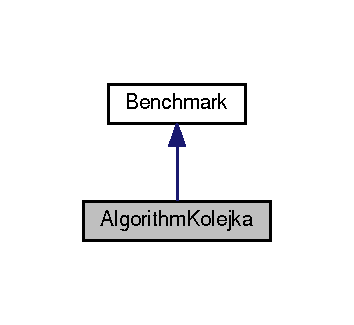
\includegraphics[width=170pt]{class_algorithm_kolejka__inherit__graph}
\end{center}
\end{figure}


Collaboration diagram for Algorithm\+Kolejka\+:\nopagebreak
\begin{figure}[H]
\begin{center}
\leavevmode
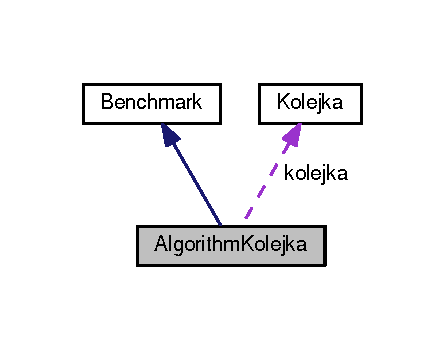
\includegraphics[width=213pt]{class_algorithm_kolejka__coll__graph}
\end{center}
\end{figure}
\subsection*{Public Member Functions}
\begin{DoxyCompactItemize}
\item 
\hyperlink{class_algorithm_kolejka_a024b4d14ce3e46ad167fa1961168088e}{Algorithm\+Kolejka} ()
\begin{DoxyCompactList}\small\item\em Konstruktor obiektu \hyperlink{class_algorithm_kolejka}{Algorithm\+Kolejka}. \end{DoxyCompactList}\item 
\hyperlink{class_algorithm_kolejka_a734671abcf48ef75dd1df980b503e618}{Algorithm\+Kolejka} (int \+\_\+tab\mbox{[}$\,$\mbox{]})
\begin{DoxyCompactList}\small\item\em Konstruktor parametryczny obiektu \hyperlink{class_algorithm_kolejka}{Algorithm\+Kolejka}. \end{DoxyCompactList}\item 
\hyperlink{class_algorithm_kolejka_a1df769a80bf632f57437c8d0cf6874d2}{$\sim$\+Algorithm\+Kolejka} ()
\begin{DoxyCompactList}\small\item\em Destruktor obiektu \hyperlink{class_algorithm_kolejka}{Algorithm\+Kolejka}. \end{DoxyCompactList}\item 
virtual void \hyperlink{class_algorithm_kolejka_ac739a8c865d4b71232549d12e0f1f466}{test\+Algorithm} (\hyperlink{class_benchmark}{Benchmark} $\ast$\+\_\+algorithm)
\begin{DoxyCompactList}\small\item\em Metoda testowania algorytmu. Metoda sluzy do testowania szybkosci dzialania algorytmu. W klasie \hyperlink{class_algorithm_kolejka}{Algorithm\+Kolejka} nie ma konkretnego dzialania. \end{DoxyCompactList}\item 
virtual void \hyperlink{class_algorithm_kolejka_ae9da3f1862fd90feb4a3c1d6b4f3dd8d}{run\+Algorithm} (int \+\_\+border)
\begin{DoxyCompactList}\small\item\em Metoda uruchamiania algorytmu. Metoda sluzy to wykonywania danego algorytmu. Wczytuje elementy do kolejki. \end{DoxyCompactList}\end{DoxyCompactItemize}
\subsection*{Private Attributes}
\begin{DoxyCompactItemize}
\item 
int \hyperlink{class_algorithm_kolejka_a12512e397f0f154464dc42fb060fdd3e}{tab} \mbox{[}\hyperlink{benchmark_8hh_a70ed59adcb4159ac551058053e649640}{S\+I\+Z\+E}\mbox{]}
\begin{DoxyCompactList}\small\item\em Tablica elementow z danymi wejsciowymi. \end{DoxyCompactList}\item 
\hyperlink{class_kolejka}{Kolejka} \hyperlink{class_algorithm_kolejka_a49a2b654776c15b98475ce3a7491c3ed}{kolejka}
\begin{DoxyCompactList}\small\item\em Zmienna przechowujaca kolejke. \end{DoxyCompactList}\end{DoxyCompactItemize}


\subsection{Detailed Description}


Definition at line 9 of file algorithm\+\_\+kolejka.\+hh.



\subsection{Constructor \& Destructor Documentation}
\hypertarget{class_algorithm_kolejka_a024b4d14ce3e46ad167fa1961168088e}{}\index{Algorithm\+Kolejka@{Algorithm\+Kolejka}!Algorithm\+Kolejka@{Algorithm\+Kolejka}}
\index{Algorithm\+Kolejka@{Algorithm\+Kolejka}!Algorithm\+Kolejka@{Algorithm\+Kolejka}}
\subsubsection[{Algorithm\+Kolejka}]{\setlength{\rightskip}{0pt plus 5cm}Algorithm\+Kolejka\+::\+Algorithm\+Kolejka (
\begin{DoxyParamCaption}
{}
\end{DoxyParamCaption}
)\hspace{0.3cm}{\ttfamily [inline]}}\label{class_algorithm_kolejka_a024b4d14ce3e46ad167fa1961168088e}


Definition at line 24 of file algorithm\+\_\+kolejka.\+hh.

\hypertarget{class_algorithm_kolejka_a734671abcf48ef75dd1df980b503e618}{}\index{Algorithm\+Kolejka@{Algorithm\+Kolejka}!Algorithm\+Kolejka@{Algorithm\+Kolejka}}
\index{Algorithm\+Kolejka@{Algorithm\+Kolejka}!Algorithm\+Kolejka@{Algorithm\+Kolejka}}
\subsubsection[{Algorithm\+Kolejka}]{\setlength{\rightskip}{0pt plus 5cm}Algorithm\+Kolejka\+::\+Algorithm\+Kolejka (
\begin{DoxyParamCaption}
\item[{int}]{\+\_\+tab\mbox{[}$\,$\mbox{]}}
\end{DoxyParamCaption}
)\hspace{0.3cm}{\ttfamily [inline]}}\label{class_algorithm_kolejka_a734671abcf48ef75dd1df980b503e618}

\begin{DoxyParams}[1]{Parameters}
\mbox{\tt in}  & {\em \+\_\+tab} & -\/ tablica przechowujaca dane wejsciowe. \\
\hline
\end{DoxyParams}


Definition at line 30 of file algorithm\+\_\+kolejka.\+hh.

\hypertarget{class_algorithm_kolejka_a1df769a80bf632f57437c8d0cf6874d2}{}\index{Algorithm\+Kolejka@{Algorithm\+Kolejka}!````~Algorithm\+Kolejka@{$\sim$\+Algorithm\+Kolejka}}
\index{````~Algorithm\+Kolejka@{$\sim$\+Algorithm\+Kolejka}!Algorithm\+Kolejka@{Algorithm\+Kolejka}}
\subsubsection[{$\sim$\+Algorithm\+Kolejka}]{\setlength{\rightskip}{0pt plus 5cm}Algorithm\+Kolejka\+::$\sim$\+Algorithm\+Kolejka (
\begin{DoxyParamCaption}
{}
\end{DoxyParamCaption}
)\hspace{0.3cm}{\ttfamily [inline]}}\label{class_algorithm_kolejka_a1df769a80bf632f57437c8d0cf6874d2}


Definition at line 35 of file algorithm\+\_\+kolejka.\+hh.



\subsection{Member Function Documentation}
\hypertarget{class_algorithm_kolejka_ae9da3f1862fd90feb4a3c1d6b4f3dd8d}{}\index{Algorithm\+Kolejka@{Algorithm\+Kolejka}!run\+Algorithm@{run\+Algorithm}}
\index{run\+Algorithm@{run\+Algorithm}!Algorithm\+Kolejka@{Algorithm\+Kolejka}}
\subsubsection[{run\+Algorithm}]{\setlength{\rightskip}{0pt plus 5cm}void Algorithm\+Kolejka\+::run\+Algorithm (
\begin{DoxyParamCaption}
\item[{int}]{\+\_\+border}
\end{DoxyParamCaption}
)\hspace{0.3cm}{\ttfamily [virtual]}}\label{class_algorithm_kolejka_ae9da3f1862fd90feb4a3c1d6b4f3dd8d}

\begin{DoxyParams}[1]{Parameters}
\mbox{\tt in}  & {\em \+\_\+border} & -\/ ilosc elementow dla ktorych algorytm ma wykonac swoje dzialanie. \\
\hline
\end{DoxyParams}


Reimplemented from \hyperlink{class_benchmark_a6363894c058e8bfe146de09d7126b29c}{Benchmark}.



Definition at line 8 of file algorithm\+\_\+kolejka.\+cpp.



Here is the call graph for this function\+:\nopagebreak
\begin{figure}[H]
\begin{center}
\leavevmode
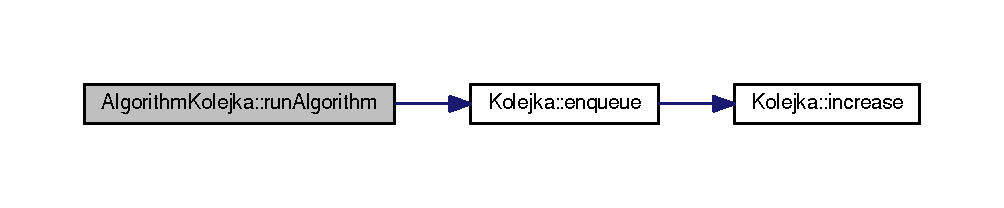
\includegraphics[width=350pt]{class_algorithm_kolejka_ae9da3f1862fd90feb4a3c1d6b4f3dd8d_cgraph}
\end{center}
\end{figure}


\hypertarget{class_algorithm_kolejka_ac739a8c865d4b71232549d12e0f1f466}{}\index{Algorithm\+Kolejka@{Algorithm\+Kolejka}!test\+Algorithm@{test\+Algorithm}}
\index{test\+Algorithm@{test\+Algorithm}!Algorithm\+Kolejka@{Algorithm\+Kolejka}}
\subsubsection[{test\+Algorithm}]{\setlength{\rightskip}{0pt plus 5cm}virtual void Algorithm\+Kolejka\+::test\+Algorithm (
\begin{DoxyParamCaption}
\item[{{\bf Benchmark} $\ast$}]{\+\_\+algorithm}
\end{DoxyParamCaption}
)\hspace{0.3cm}{\ttfamily [inline]}, {\ttfamily [virtual]}}\label{class_algorithm_kolejka_ac739a8c865d4b71232549d12e0f1f466}

\begin{DoxyParams}[1]{Parameters}
\mbox{\tt in}  & {\em \+\_\+algorithm} & -\/ testowany algorytm. \\
\hline
\end{DoxyParams}


Definition at line 43 of file algorithm\+\_\+kolejka.\+hh.



\subsection{Member Data Documentation}
\hypertarget{class_algorithm_kolejka_a49a2b654776c15b98475ce3a7491c3ed}{}\index{Algorithm\+Kolejka@{Algorithm\+Kolejka}!kolejka@{kolejka}}
\index{kolejka@{kolejka}!Algorithm\+Kolejka@{Algorithm\+Kolejka}}
\subsubsection[{kolejka}]{\setlength{\rightskip}{0pt plus 5cm}{\bf Kolejka} Algorithm\+Kolejka\+::kolejka\hspace{0.3cm}{\ttfamily [private]}}\label{class_algorithm_kolejka_a49a2b654776c15b98475ce3a7491c3ed}


Definition at line 18 of file algorithm\+\_\+kolejka.\+hh.

\hypertarget{class_algorithm_kolejka_a12512e397f0f154464dc42fb060fdd3e}{}\index{Algorithm\+Kolejka@{Algorithm\+Kolejka}!tab@{tab}}
\index{tab@{tab}!Algorithm\+Kolejka@{Algorithm\+Kolejka}}
\subsubsection[{tab}]{\setlength{\rightskip}{0pt plus 5cm}int Algorithm\+Kolejka\+::tab\mbox{[}{\bf S\+I\+Z\+E}\mbox{]}\hspace{0.3cm}{\ttfamily [private]}}\label{class_algorithm_kolejka_a12512e397f0f154464dc42fb060fdd3e}


Definition at line 14 of file algorithm\+\_\+kolejka.\+hh.



The documentation for this class was generated from the following files\+:\begin{DoxyCompactItemize}
\item 
\hyperlink{algorithm__kolejka_8hh}{algorithm\+\_\+kolejka.\+hh}\item 
\hyperlink{algorithm__kolejka_8cpp}{algorithm\+\_\+kolejka.\+cpp}\end{DoxyCompactItemize}

\hypertarget{class_algorithm_lista}{\section{Algorithm\-Lista Class Reference}
\label{class_algorithm_lista}\index{Algorithm\-Lista@{Algorithm\-Lista}}
}


Klasa \hyperlink{class_algorithm_lista}{Algorithm\-Lista} modelujaca algorytm wczytywania do kolejki. Obiekt tego typu reprezentuje algorytm wykonujacy wykonujacy wczytywanie zadanej ilosci elementow do listy.  




{\ttfamily \#include $<$algorithm\-\_\-lista.\-hh$>$}



Inheritance diagram for Algorithm\-Lista\-:\nopagebreak
\begin{figure}[H]
\begin{center}
\leavevmode
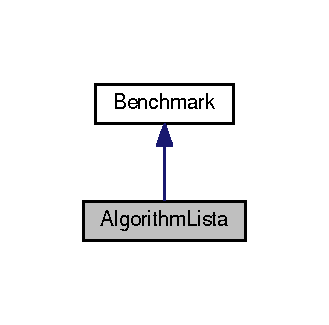
\includegraphics[width=160pt]{class_algorithm_lista__inherit__graph}
\end{center}
\end{figure}


Collaboration diagram for Algorithm\-Lista\-:\nopagebreak
\begin{figure}[H]
\begin{center}
\leavevmode
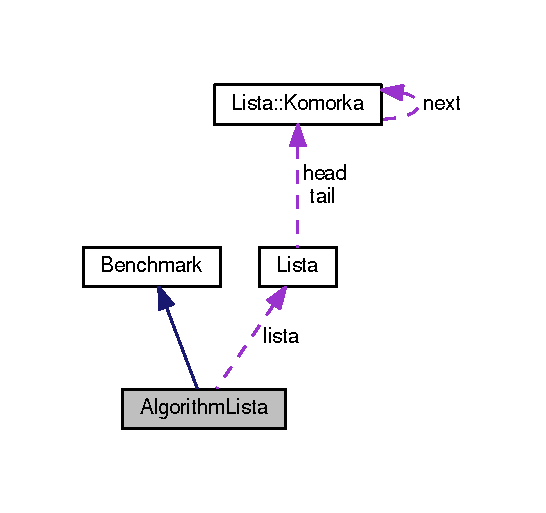
\includegraphics[width=263pt]{class_algorithm_lista__coll__graph}
\end{center}
\end{figure}
\subsection*{Public Member Functions}
\begin{DoxyCompactItemize}
\item 
\hyperlink{class_algorithm_lista_a4c7749379de38154982288419f305141}{Algorithm\-Lista} ()
\begin{DoxyCompactList}\small\item\em Konstruktor obiektu \hyperlink{class_algorithm_lista}{Algorithm\-Lista}. \end{DoxyCompactList}\item 
\hyperlink{class_algorithm_lista_ab5aed5527ca4f27c213e97fa19f6e32d}{Algorithm\-Lista} (int \-\_\-tab\mbox{[}$\,$\mbox{]})
\begin{DoxyCompactList}\small\item\em Konstruktor parametryczny obiektu \hyperlink{class_algorithm_lista}{Algorithm\-Lista}. \end{DoxyCompactList}\item 
\hyperlink{class_algorithm_lista_a2d7c5ef95cdfe523a86b01da06d0fb2e}{$\sim$\-Algorithm\-Lista} ()
\begin{DoxyCompactList}\small\item\em Destruktor obiektu \hyperlink{class_algorithm_lista}{Algorithm\-Lista}. \end{DoxyCompactList}\item 
virtual void \hyperlink{class_algorithm_lista_a1e1f93e75b4a635098bf30ec32f19903}{test\-Algorithm} (\hyperlink{class_benchmark}{Benchmark} $\ast$\-\_\-algorithm)
\begin{DoxyCompactList}\small\item\em Metoda testowania algorytmu. Metoda sluzy do testowania szybkosci dzialania algorytmu. W klasie \hyperlink{class_algorithm_lista}{Algorithm\-Lista} nie ma konkretnego dzialania. \end{DoxyCompactList}\item 
virtual void \hyperlink{class_algorithm_lista_a5c41dbbd3ae7a9ac34edec1a51bc8eb1}{run\-Algorithm} (int \-\_\-border)
\begin{DoxyCompactList}\small\item\em Metoda uruchamiania algorytmu. Metoda sluzy to wykonywania danego algorytmu. Wczytuje elementy do kolejki. \end{DoxyCompactList}\end{DoxyCompactItemize}
\subsection*{Private Attributes}
\begin{DoxyCompactItemize}
\item 
int \hyperlink{class_algorithm_lista_ad04d74953d75c8886b0c5cfda71773f7}{tab} \mbox{[}\hyperlink{benchmark_8hh_a70ed59adcb4159ac551058053e649640}{S\-I\-Z\-E}\mbox{]}
\begin{DoxyCompactList}\small\item\em Tablica elementow z danymi wejsciowymi. \end{DoxyCompactList}\item 
\hyperlink{class_lista}{Lista} \hyperlink{class_algorithm_lista_a5c4c8b55e6d71eae06c98cd39f38bb30}{lista}
\begin{DoxyCompactList}\small\item\em Zmienna przechowujaca liste. \end{DoxyCompactList}\end{DoxyCompactItemize}


\subsection{Detailed Description}


Definition at line 9 of file algorithm\-\_\-lista.\-hh.



\subsection{Constructor \& Destructor Documentation}
\hypertarget{class_algorithm_lista_a4c7749379de38154982288419f305141}{\index{Algorithm\-Lista@{Algorithm\-Lista}!Algorithm\-Lista@{Algorithm\-Lista}}
\index{Algorithm\-Lista@{Algorithm\-Lista}!AlgorithmLista@{Algorithm\-Lista}}
\subsubsection[{Algorithm\-Lista}]{\setlength{\rightskip}{0pt plus 5cm}Algorithm\-Lista\-::\-Algorithm\-Lista (
\begin{DoxyParamCaption}
{}
\end{DoxyParamCaption}
)\hspace{0.3cm}{\ttfamily [inline]}}}\label{class_algorithm_lista_a4c7749379de38154982288419f305141}


Definition at line 24 of file algorithm\-\_\-lista.\-hh.

\hypertarget{class_algorithm_lista_ab5aed5527ca4f27c213e97fa19f6e32d}{\index{Algorithm\-Lista@{Algorithm\-Lista}!Algorithm\-Lista@{Algorithm\-Lista}}
\index{Algorithm\-Lista@{Algorithm\-Lista}!AlgorithmLista@{Algorithm\-Lista}}
\subsubsection[{Algorithm\-Lista}]{\setlength{\rightskip}{0pt plus 5cm}Algorithm\-Lista\-::\-Algorithm\-Lista (
\begin{DoxyParamCaption}
\item[{int}]{\-\_\-tab\mbox{[}$\,$\mbox{]}}
\end{DoxyParamCaption}
)\hspace{0.3cm}{\ttfamily [inline]}}}\label{class_algorithm_lista_ab5aed5527ca4f27c213e97fa19f6e32d}

\begin{DoxyParams}[1]{Parameters}
\mbox{\tt in}  & {\em \-\_\-tab} & -\/ tablica przechowujaca dane wejsciowe. \\
\hline
\end{DoxyParams}


Definition at line 30 of file algorithm\-\_\-lista.\-hh.

\hypertarget{class_algorithm_lista_a2d7c5ef95cdfe523a86b01da06d0fb2e}{\index{Algorithm\-Lista@{Algorithm\-Lista}!$\sim$\-Algorithm\-Lista@{$\sim$\-Algorithm\-Lista}}
\index{$\sim$\-Algorithm\-Lista@{$\sim$\-Algorithm\-Lista}!AlgorithmLista@{Algorithm\-Lista}}
\subsubsection[{$\sim$\-Algorithm\-Lista}]{\setlength{\rightskip}{0pt plus 5cm}Algorithm\-Lista\-::$\sim$\-Algorithm\-Lista (
\begin{DoxyParamCaption}
{}
\end{DoxyParamCaption}
)\hspace{0.3cm}{\ttfamily [inline]}}}\label{class_algorithm_lista_a2d7c5ef95cdfe523a86b01da06d0fb2e}


Definition at line 35 of file algorithm\-\_\-lista.\-hh.



\subsection{Member Function Documentation}
\hypertarget{class_algorithm_lista_a5c41dbbd3ae7a9ac34edec1a51bc8eb1}{\index{Algorithm\-Lista@{Algorithm\-Lista}!run\-Algorithm@{run\-Algorithm}}
\index{run\-Algorithm@{run\-Algorithm}!AlgorithmLista@{Algorithm\-Lista}}
\subsubsection[{run\-Algorithm}]{\setlength{\rightskip}{0pt plus 5cm}void Algorithm\-Lista\-::run\-Algorithm (
\begin{DoxyParamCaption}
\item[{int}]{\-\_\-border}
\end{DoxyParamCaption}
)\hspace{0.3cm}{\ttfamily [virtual]}}}\label{class_algorithm_lista_a5c41dbbd3ae7a9ac34edec1a51bc8eb1}

\begin{DoxyParams}[1]{Parameters}
\mbox{\tt in}  & {\em \-\_\-border} & -\/ ilosc elementow dla ktorych algorytm ma wykonac swoje dzialanie. \\
\hline
\end{DoxyParams}


Reimplemented from \hyperlink{class_benchmark_a6363894c058e8bfe146de09d7126b29c}{Benchmark}.



Definition at line 8 of file algorithm\-\_\-lista.\-cpp.



Here is the call graph for this function\-:\nopagebreak
\begin{figure}[H]
\begin{center}
\leavevmode
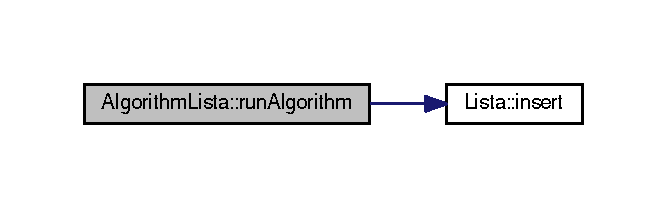
\includegraphics[width=324pt]{class_algorithm_lista_a5c41dbbd3ae7a9ac34edec1a51bc8eb1_cgraph}
\end{center}
\end{figure}


\hypertarget{class_algorithm_lista_a1e1f93e75b4a635098bf30ec32f19903}{\index{Algorithm\-Lista@{Algorithm\-Lista}!test\-Algorithm@{test\-Algorithm}}
\index{test\-Algorithm@{test\-Algorithm}!AlgorithmLista@{Algorithm\-Lista}}
\subsubsection[{test\-Algorithm}]{\setlength{\rightskip}{0pt plus 5cm}virtual void Algorithm\-Lista\-::test\-Algorithm (
\begin{DoxyParamCaption}
\item[{{\bf Benchmark} $\ast$}]{\-\_\-algorithm}
\end{DoxyParamCaption}
)\hspace{0.3cm}{\ttfamily [inline]}, {\ttfamily [virtual]}}}\label{class_algorithm_lista_a1e1f93e75b4a635098bf30ec32f19903}

\begin{DoxyParams}[1]{Parameters}
\mbox{\tt in}  & {\em \-\_\-algorithm} & -\/ testowany algorytm. \\
\hline
\end{DoxyParams}


Definition at line 43 of file algorithm\-\_\-lista.\-hh.



\subsection{Member Data Documentation}
\hypertarget{class_algorithm_lista_a5c4c8b55e6d71eae06c98cd39f38bb30}{\index{Algorithm\-Lista@{Algorithm\-Lista}!lista@{lista}}
\index{lista@{lista}!AlgorithmLista@{Algorithm\-Lista}}
\subsubsection[{lista}]{\setlength{\rightskip}{0pt plus 5cm}{\bf Lista} Algorithm\-Lista\-::lista\hspace{0.3cm}{\ttfamily [private]}}}\label{class_algorithm_lista_a5c4c8b55e6d71eae06c98cd39f38bb30}


Definition at line 18 of file algorithm\-\_\-lista.\-hh.

\hypertarget{class_algorithm_lista_ad04d74953d75c8886b0c5cfda71773f7}{\index{Algorithm\-Lista@{Algorithm\-Lista}!tab@{tab}}
\index{tab@{tab}!AlgorithmLista@{Algorithm\-Lista}}
\subsubsection[{tab}]{\setlength{\rightskip}{0pt plus 5cm}int Algorithm\-Lista\-::tab\mbox{[}{\bf S\-I\-Z\-E}\mbox{]}\hspace{0.3cm}{\ttfamily [private]}}}\label{class_algorithm_lista_ad04d74953d75c8886b0c5cfda71773f7}


Definition at line 14 of file algorithm\-\_\-lista.\-hh.



The documentation for this class was generated from the following files\-:\begin{DoxyCompactItemize}
\item 
\hyperlink{algorithm__lista_8hh}{algorithm\-\_\-lista.\-hh}\item 
\hyperlink{algorithm__lista_8cpp}{algorithm\-\_\-lista.\-cpp}\end{DoxyCompactItemize}

\hypertarget{class_algorithm_stos}{}\section{Algorithm\+Stos Class Reference}
\label{class_algorithm_stos}\index{Algorithm\+Stos@{Algorithm\+Stos}}


Klasa \hyperlink{class_algorithm_stos}{Algorithm\+Stos} modelujaca algorytm wczytywania do stosu. Obiekt tego typu reprezentuje algorytm wykonujacy wykonujacy wczytywanie zadanej ilosci elementow do stosu.  




{\ttfamily \#include $<$algorithm\+\_\+stos.\+hh$>$}



Inheritance diagram for Algorithm\+Stos\+:\nopagebreak
\begin{figure}[H]
\begin{center}
\leavevmode
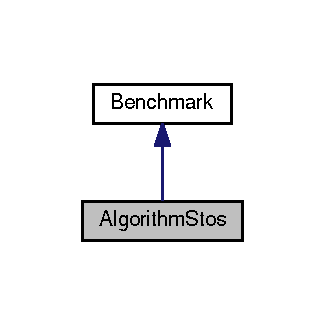
\includegraphics[width=156pt]{class_algorithm_stos__inherit__graph}
\end{center}
\end{figure}


Collaboration diagram for Algorithm\+Stos\+:\nopagebreak
\begin{figure}[H]
\begin{center}
\leavevmode
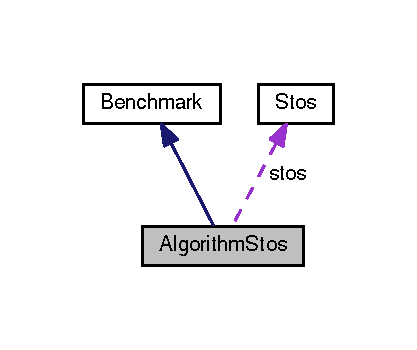
\includegraphics[width=200pt]{class_algorithm_stos__coll__graph}
\end{center}
\end{figure}
\subsection*{Public Member Functions}
\begin{DoxyCompactItemize}
\item 
\hyperlink{class_algorithm_stos_a0d987377d7c5d9cea3152680ba437cd3}{Algorithm\+Stos} ()
\begin{DoxyCompactList}\small\item\em Konstruktor obiektu \hyperlink{class_algorithm_stos}{Algorithm\+Stos}. \end{DoxyCompactList}\item 
\hyperlink{class_algorithm_stos_a5dc7ad87d403c67d64aa6cac6a626992}{Algorithm\+Stos} (int \+\_\+tab\mbox{[}$\,$\mbox{]})
\begin{DoxyCompactList}\small\item\em Konstruktor parametryczny obiektu \hyperlink{class_algorithm_stos}{Algorithm\+Stos}. \end{DoxyCompactList}\item 
\hyperlink{class_algorithm_stos_a68a3733d5dfd9fefe38059f0ce0202bf}{$\sim$\+Algorithm\+Stos} ()
\begin{DoxyCompactList}\small\item\em Destruktor obiektu \hyperlink{class_algorithm_stos}{Algorithm\+Stos}. \end{DoxyCompactList}\item 
virtual void \hyperlink{class_algorithm_stos_a7fb987baf970d51f90ad880d27e537a4}{test\+Algorithm} (\hyperlink{class_benchmark}{Benchmark} $\ast$\+\_\+algorithm)
\begin{DoxyCompactList}\small\item\em Metoda testowania algorytmu. Metoda sluzy do testowania szybkosci dzialania algorytmu. W klasie \hyperlink{class_algorithm_stos}{Algorithm\+Stos} nie ma konkretnego dzialania. \end{DoxyCompactList}\item 
virtual void \hyperlink{class_algorithm_stos_a889f7150ae3651b40e5acca7542dbbd1}{run\+Algorithm} (int \+\_\+border)
\begin{DoxyCompactList}\small\item\em Metoda uruchamiania algorytmu. Metoda sluzy to wykonywania danego algorytmu. Wczytuje elementy do stosu. \end{DoxyCompactList}\end{DoxyCompactItemize}
\subsection*{Private Attributes}
\begin{DoxyCompactItemize}
\item 
int \hyperlink{class_algorithm_stos_a2fb5db929aa54bf64794c812830d8648}{tab} \mbox{[}\hyperlink{benchmark_8hh_a70ed59adcb4159ac551058053e649640}{S\+I\+Z\+E}\mbox{]}
\begin{DoxyCompactList}\small\item\em Tablica elementow z danymi wejsciowymi. \end{DoxyCompactList}\item 
\hyperlink{class_stos}{Stos} \hyperlink{class_algorithm_stos_a0b803ecc25fd3586cf07969697367754}{stos}
\begin{DoxyCompactList}\small\item\em Zmienna przechowujaca stos. \end{DoxyCompactList}\end{DoxyCompactItemize}


\subsection{Detailed Description}


Definition at line 9 of file algorithm\+\_\+stos.\+hh.



\subsection{Constructor \& Destructor Documentation}
\hypertarget{class_algorithm_stos_a0d987377d7c5d9cea3152680ba437cd3}{}\index{Algorithm\+Stos@{Algorithm\+Stos}!Algorithm\+Stos@{Algorithm\+Stos}}
\index{Algorithm\+Stos@{Algorithm\+Stos}!Algorithm\+Stos@{Algorithm\+Stos}}
\subsubsection[{Algorithm\+Stos}]{\setlength{\rightskip}{0pt plus 5cm}Algorithm\+Stos\+::\+Algorithm\+Stos (
\begin{DoxyParamCaption}
{}
\end{DoxyParamCaption}
)\hspace{0.3cm}{\ttfamily [inline]}}\label{class_algorithm_stos_a0d987377d7c5d9cea3152680ba437cd3}


Definition at line 24 of file algorithm\+\_\+stos.\+hh.

\hypertarget{class_algorithm_stos_a5dc7ad87d403c67d64aa6cac6a626992}{}\index{Algorithm\+Stos@{Algorithm\+Stos}!Algorithm\+Stos@{Algorithm\+Stos}}
\index{Algorithm\+Stos@{Algorithm\+Stos}!Algorithm\+Stos@{Algorithm\+Stos}}
\subsubsection[{Algorithm\+Stos}]{\setlength{\rightskip}{0pt plus 5cm}Algorithm\+Stos\+::\+Algorithm\+Stos (
\begin{DoxyParamCaption}
\item[{int}]{\+\_\+tab\mbox{[}$\,$\mbox{]}}
\end{DoxyParamCaption}
)\hspace{0.3cm}{\ttfamily [inline]}}\label{class_algorithm_stos_a5dc7ad87d403c67d64aa6cac6a626992}

\begin{DoxyParams}[1]{Parameters}
\mbox{\tt in}  & {\em \+\_\+tab} & -\/ tablica przechowujaca dane wejsciowe. \\
\hline
\end{DoxyParams}


Definition at line 30 of file algorithm\+\_\+stos.\+hh.

\hypertarget{class_algorithm_stos_a68a3733d5dfd9fefe38059f0ce0202bf}{}\index{Algorithm\+Stos@{Algorithm\+Stos}!````~Algorithm\+Stos@{$\sim$\+Algorithm\+Stos}}
\index{````~Algorithm\+Stos@{$\sim$\+Algorithm\+Stos}!Algorithm\+Stos@{Algorithm\+Stos}}
\subsubsection[{$\sim$\+Algorithm\+Stos}]{\setlength{\rightskip}{0pt plus 5cm}Algorithm\+Stos\+::$\sim$\+Algorithm\+Stos (
\begin{DoxyParamCaption}
{}
\end{DoxyParamCaption}
)\hspace{0.3cm}{\ttfamily [inline]}}\label{class_algorithm_stos_a68a3733d5dfd9fefe38059f0ce0202bf}


Definition at line 35 of file algorithm\+\_\+stos.\+hh.



\subsection{Member Function Documentation}
\hypertarget{class_algorithm_stos_a889f7150ae3651b40e5acca7542dbbd1}{}\index{Algorithm\+Stos@{Algorithm\+Stos}!run\+Algorithm@{run\+Algorithm}}
\index{run\+Algorithm@{run\+Algorithm}!Algorithm\+Stos@{Algorithm\+Stos}}
\subsubsection[{run\+Algorithm}]{\setlength{\rightskip}{0pt plus 5cm}void Algorithm\+Stos\+::run\+Algorithm (
\begin{DoxyParamCaption}
\item[{int}]{\+\_\+border}
\end{DoxyParamCaption}
)\hspace{0.3cm}{\ttfamily [virtual]}}\label{class_algorithm_stos_a889f7150ae3651b40e5acca7542dbbd1}

\begin{DoxyParams}[1]{Parameters}
\mbox{\tt in}  & {\em \+\_\+border} & -\/ ilosc elementow dla ktorych algorytm ma wykonac swoje dzialanie. \\
\hline
\end{DoxyParams}


Reimplemented from \hyperlink{class_benchmark_a6363894c058e8bfe146de09d7126b29c}{Benchmark}.



Definition at line 8 of file algorithm\+\_\+stos.\+cpp.



Here is the call graph for this function\+:\nopagebreak
\begin{figure}[H]
\begin{center}
\leavevmode
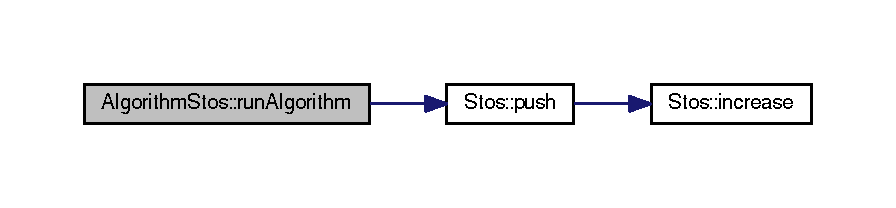
\includegraphics[width=350pt]{class_algorithm_stos_a889f7150ae3651b40e5acca7542dbbd1_cgraph}
\end{center}
\end{figure}


\hypertarget{class_algorithm_stos_a7fb987baf970d51f90ad880d27e537a4}{}\index{Algorithm\+Stos@{Algorithm\+Stos}!test\+Algorithm@{test\+Algorithm}}
\index{test\+Algorithm@{test\+Algorithm}!Algorithm\+Stos@{Algorithm\+Stos}}
\subsubsection[{test\+Algorithm}]{\setlength{\rightskip}{0pt plus 5cm}virtual void Algorithm\+Stos\+::test\+Algorithm (
\begin{DoxyParamCaption}
\item[{{\bf Benchmark} $\ast$}]{\+\_\+algorithm}
\end{DoxyParamCaption}
)\hspace{0.3cm}{\ttfamily [inline]}, {\ttfamily [virtual]}}\label{class_algorithm_stos_a7fb987baf970d51f90ad880d27e537a4}

\begin{DoxyParams}[1]{Parameters}
\mbox{\tt in}  & {\em \+\_\+algorithm} & -\/ testowany algorytm. \\
\hline
\end{DoxyParams}


Definition at line 43 of file algorithm\+\_\+stos.\+hh.



\subsection{Member Data Documentation}
\hypertarget{class_algorithm_stos_a0b803ecc25fd3586cf07969697367754}{}\index{Algorithm\+Stos@{Algorithm\+Stos}!stos@{stos}}
\index{stos@{stos}!Algorithm\+Stos@{Algorithm\+Stos}}
\subsubsection[{stos}]{\setlength{\rightskip}{0pt plus 5cm}{\bf Stos} Algorithm\+Stos\+::stos\hspace{0.3cm}{\ttfamily [private]}}\label{class_algorithm_stos_a0b803ecc25fd3586cf07969697367754}


Definition at line 18 of file algorithm\+\_\+stos.\+hh.

\hypertarget{class_algorithm_stos_a2fb5db929aa54bf64794c812830d8648}{}\index{Algorithm\+Stos@{Algorithm\+Stos}!tab@{tab}}
\index{tab@{tab}!Algorithm\+Stos@{Algorithm\+Stos}}
\subsubsection[{tab}]{\setlength{\rightskip}{0pt plus 5cm}int Algorithm\+Stos\+::tab\mbox{[}{\bf S\+I\+Z\+E}\mbox{]}\hspace{0.3cm}{\ttfamily [private]}}\label{class_algorithm_stos_a2fb5db929aa54bf64794c812830d8648}


Definition at line 14 of file algorithm\+\_\+stos.\+hh.



The documentation for this class was generated from the following files\+:\begin{DoxyCompactItemize}
\item 
\hyperlink{algorithm__stos_8hh}{algorithm\+\_\+stos.\+hh}\item 
\hyperlink{algorithm__stos_8cpp}{algorithm\+\_\+stos.\+cpp}\end{DoxyCompactItemize}

\hypertarget{class_benchmark}{}\section{Benchmark Class Reference}
\label{class_benchmark}\index{Benchmark@{Benchmark}}


Klasa \hyperlink{class_benchmark}{Benchmark} modelujaca program benchmarkujacy. Obiekt tego typu reprezentuje program sprawdzajacy szybkosc wykonywania algorytmow.  




{\ttfamily \#include $<$benchmark.\+hh$>$}



Inheritance diagram for Benchmark\+:\nopagebreak
\begin{figure}[H]
\begin{center}
\leavevmode
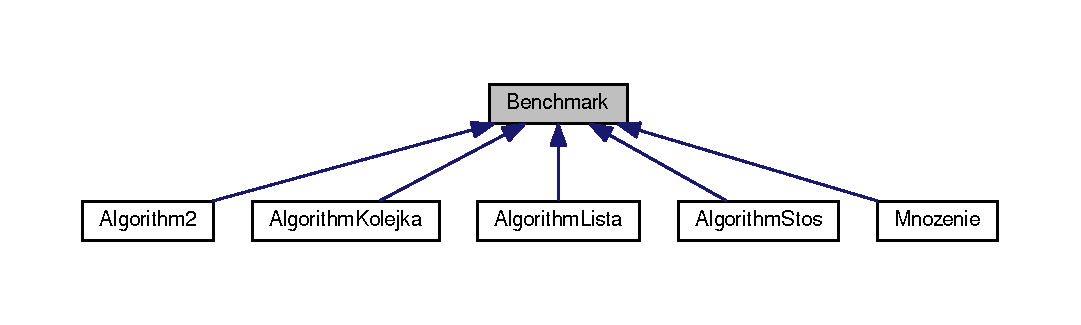
\includegraphics[width=350pt]{class_benchmark__inherit__graph}
\end{center}
\end{figure}
\subsection*{Public Member Functions}
\begin{DoxyCompactItemize}
\item 
\hyperlink{class_benchmark_acfca497989836a688d44477802e822d8}{Benchmark} ()
\begin{DoxyCompactList}\small\item\em Konstrukor obiektu \hyperlink{class_benchmark}{Benchmark}. \end{DoxyCompactList}\item 
\hyperlink{class_benchmark_a20476e07f09e2b20ed3e9a7f13a570e6}{$\sim$\+Benchmark} ()
\begin{DoxyCompactList}\small\item\em Destruktor obiektu \hyperlink{class_benchmark}{Benchmark}. \end{DoxyCompactList}\item 
virtual void \hyperlink{class_benchmark_a900bc0d26c2ed6aa45afe4d5b295ccd1}{test\+Algorithm} (\hyperlink{class_benchmark}{Benchmark} $\ast$\+\_\+algorithm, int \+\_\+n) const 
\begin{DoxyCompactList}\small\item\em Metoda testowania algorytmu. Metoda sluzy to testowania szybkosci dzialania algorytmu. Wykonuje testowany algorytm dla 5 kolejnych ilosci elementow. Wykonanie algorytmu dla danego zestawu liczb powtarza dwa razy i usrednia wynik. Otrzymany czas wraz z iloscia testowanych danych zapisuje w pliku ret\+\_\+data.\+txt. \end{DoxyCompactList}\item 
virtual void \hyperlink{class_benchmark_a6363894c058e8bfe146de09d7126b29c}{run\+Algorithm} (int \+\_\+border)
\begin{DoxyCompactList}\small\item\em Metoda uruchamiania algorytmu. Metoda sluzy do wykonywania danego algorytmu. W klasie \hyperlink{class_benchmark}{Benchmark} nie ma konkretnego dzialania. \end{DoxyCompactList}\item 
virtual void \hyperlink{class_benchmark_a05a8e8b9b80949f51c2ccc47e08dedbb}{run\+Algorithm\+Szybkie\+Sortowanie} ()
\begin{DoxyCompactList}\small\item\em Metoda uruchamiania algorytmu szybkiego sortowania. Metoda sluzy do wykonywania danego algorytmu. W klasie \hyperlink{class_benchmark}{Benchmark} nie ma konkretnego dzialania. \end{DoxyCompactList}\end{DoxyCompactItemize}
\subsection*{Private Attributes}
\begin{DoxyCompactItemize}
\item 
std\+::string \hyperlink{class_benchmark_aee0beda65009e7334d34c5957f78c49a}{nazwy} \mbox{[}4\mbox{]} = \{\char`\"{}ret\+\_\+data1.\+txt\char`\"{}, \char`\"{}ret\+\_\+data2.\+txt\char`\"{}, \char`\"{}ret\+\_\+data3.\+txt\char`\"{}, \char`\"{}ret\+\_\+data4.\+txt\char`\"{}\}
\begin{DoxyCompactList}\small\item\em Tablica stringow przechowujaca nazwy plikow do zapisu. \end{DoxyCompactList}\end{DoxyCompactItemize}


\subsection{Detailed Description}


Definition at line 11 of file benchmark.\+hh.



\subsection{Constructor \& Destructor Documentation}
\hypertarget{class_benchmark_acfca497989836a688d44477802e822d8}{}\index{Benchmark@{Benchmark}!Benchmark@{Benchmark}}
\index{Benchmark@{Benchmark}!Benchmark@{Benchmark}}
\subsubsection[{Benchmark}]{\setlength{\rightskip}{0pt plus 5cm}Benchmark\+::\+Benchmark (
\begin{DoxyParamCaption}
{}
\end{DoxyParamCaption}
)\hspace{0.3cm}{\ttfamily [inline]}}\label{class_benchmark_acfca497989836a688d44477802e822d8}


Definition at line 23 of file benchmark.\+hh.

\hypertarget{class_benchmark_a20476e07f09e2b20ed3e9a7f13a570e6}{}\index{Benchmark@{Benchmark}!````~Benchmark@{$\sim$\+Benchmark}}
\index{````~Benchmark@{$\sim$\+Benchmark}!Benchmark@{Benchmark}}
\subsubsection[{$\sim$\+Benchmark}]{\setlength{\rightskip}{0pt plus 5cm}Benchmark\+::$\sim$\+Benchmark (
\begin{DoxyParamCaption}
{}
\end{DoxyParamCaption}
)\hspace{0.3cm}{\ttfamily [inline]}}\label{class_benchmark_a20476e07f09e2b20ed3e9a7f13a570e6}


Definition at line 28 of file benchmark.\+hh.



\subsection{Member Function Documentation}
\hypertarget{class_benchmark_a6363894c058e8bfe146de09d7126b29c}{}\index{Benchmark@{Benchmark}!run\+Algorithm@{run\+Algorithm}}
\index{run\+Algorithm@{run\+Algorithm}!Benchmark@{Benchmark}}
\subsubsection[{run\+Algorithm}]{\setlength{\rightskip}{0pt plus 5cm}virtual void Benchmark\+::run\+Algorithm (
\begin{DoxyParamCaption}
\item[{int}]{\+\_\+border}
\end{DoxyParamCaption}
)\hspace{0.3cm}{\ttfamily [inline]}, {\ttfamily [virtual]}}\label{class_benchmark_a6363894c058e8bfe146de09d7126b29c}


Reimplemented in \hyperlink{class_algorithm2_a409e58d5fb0b6d2407cc986cf163703b}{Algorithm2}, \hyperlink{class_algorithm_kolejka_ae9da3f1862fd90feb4a3c1d6b4f3dd8d}{Algorithm\+Kolejka}, \hyperlink{class_algorithm_lista_a5c41dbbd3ae7a9ac34edec1a51bc8eb1}{Algorithm\+Lista}, \hyperlink{class_algorithm_stos_a889f7150ae3651b40e5acca7542dbbd1}{Algorithm\+Stos}, and \hyperlink{class_mnozenie_a46b1c55b7ba208fa137065147e107be9}{Mnozenie}.



Definition at line 47 of file benchmark.\+hh.



Here is the caller graph for this function\+:\nopagebreak
\begin{figure}[H]
\begin{center}
\leavevmode
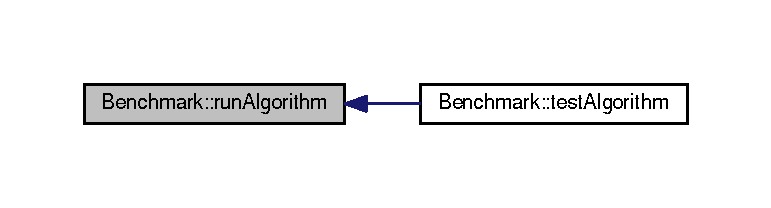
\includegraphics[width=350pt]{class_benchmark_a6363894c058e8bfe146de09d7126b29c_icgraph}
\end{center}
\end{figure}


\hypertarget{class_benchmark_a05a8e8b9b80949f51c2ccc47e08dedbb}{}\index{Benchmark@{Benchmark}!run\+Algorithm\+Szybkie\+Sortowanie@{run\+Algorithm\+Szybkie\+Sortowanie}}
\index{run\+Algorithm\+Szybkie\+Sortowanie@{run\+Algorithm\+Szybkie\+Sortowanie}!Benchmark@{Benchmark}}
\subsubsection[{run\+Algorithm\+Szybkie\+Sortowanie}]{\setlength{\rightskip}{0pt plus 5cm}virtual void Benchmark\+::run\+Algorithm\+Szybkie\+Sortowanie (
\begin{DoxyParamCaption}
{}
\end{DoxyParamCaption}
)\hspace{0.3cm}{\ttfamily [inline]}, {\ttfamily [virtual]}}\label{class_benchmark_a05a8e8b9b80949f51c2ccc47e08dedbb}


Reimplemented in \hyperlink{class_algorithm2_a103c600d6f7a33872672e4b26d89475f}{Algorithm2}.



Definition at line 54 of file benchmark.\+hh.



Here is the caller graph for this function\+:\nopagebreak
\begin{figure}[H]
\begin{center}
\leavevmode
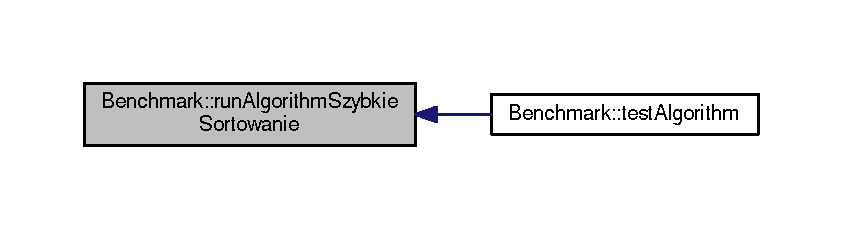
\includegraphics[width=350pt]{class_benchmark_a05a8e8b9b80949f51c2ccc47e08dedbb_icgraph}
\end{center}
\end{figure}


\hypertarget{class_benchmark_a900bc0d26c2ed6aa45afe4d5b295ccd1}{}\index{Benchmark@{Benchmark}!test\+Algorithm@{test\+Algorithm}}
\index{test\+Algorithm@{test\+Algorithm}!Benchmark@{Benchmark}}
\subsubsection[{test\+Algorithm}]{\setlength{\rightskip}{0pt plus 5cm}void Benchmark\+::test\+Algorithm (
\begin{DoxyParamCaption}
\item[{{\bf Benchmark} $\ast$}]{\+\_\+algorithm, }
\item[{int}]{\+\_\+n}
\end{DoxyParamCaption}
) const\hspace{0.3cm}{\ttfamily [virtual]}}\label{class_benchmark_a900bc0d26c2ed6aa45afe4d5b295ccd1}

\begin{DoxyParams}[1]{Parameters}
\mbox{\tt in}  & {\em \+\_\+algorithm} & -\/ testowany algorytm. \\
\hline
\mbox{\tt in}  & {\em \+\_\+n} & -\/ indeks nazwy pliku \\
\hline
\end{DoxyParams}


Definition at line 11 of file benchmark.\+cpp.



Here is the call graph for this function\+:\nopagebreak
\begin{figure}[H]
\begin{center}
\leavevmode
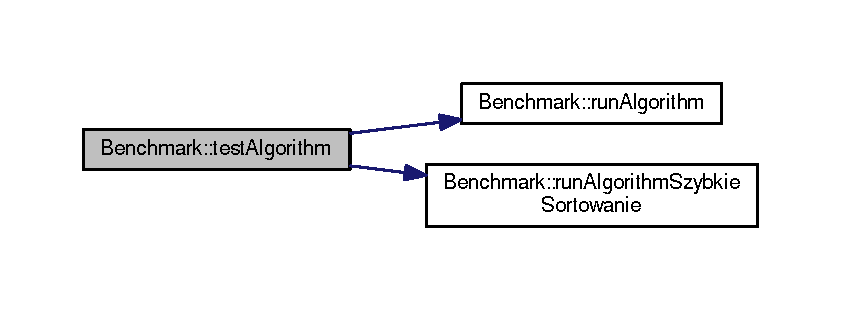
\includegraphics[width=350pt]{class_benchmark_a900bc0d26c2ed6aa45afe4d5b295ccd1_cgraph}
\end{center}
\end{figure}




\subsection{Member Data Documentation}
\hypertarget{class_benchmark_aee0beda65009e7334d34c5957f78c49a}{}\index{Benchmark@{Benchmark}!nazwy@{nazwy}}
\index{nazwy@{nazwy}!Benchmark@{Benchmark}}
\subsubsection[{nazwy}]{\setlength{\rightskip}{0pt plus 5cm}std\+::string Benchmark\+::nazwy\mbox{[}4\mbox{]} = \{\char`\"{}ret\+\_\+data1.\+txt\char`\"{}, \char`\"{}ret\+\_\+data2.\+txt\char`\"{}, \char`\"{}ret\+\_\+data3.\+txt\char`\"{}, \char`\"{}ret\+\_\+data4.\+txt\char`\"{}\}\hspace{0.3cm}{\ttfamily [private]}}\label{class_benchmark_aee0beda65009e7334d34c5957f78c49a}


Definition at line 16 of file benchmark.\+hh.



The documentation for this class was generated from the following files\+:\begin{DoxyCompactItemize}
\item 
\hyperlink{benchmark_8hh}{benchmark.\+hh}\item 
\hyperlink{benchmark_8cpp}{benchmark.\+cpp}\end{DoxyCompactItemize}

\hypertarget{class_kolejka}{\section{Kolejka Class Reference}
\label{class_kolejka}\index{Kolejka@{Kolejka}}
}


Klasa \hyperlink{class_kolejka}{Kolejka} modelujaca strukture danych typu kolejka. Obiekt tego typu reprezentuje strukture danych typu kolejka wraz z operacjami mozliwymi do wykonania na tej strukturze.  




{\ttfamily \#include $<$kolejka.\-hh$>$}

\subsection*{Public Member Functions}
\begin{DoxyCompactItemize}
\item 
\hyperlink{class_kolejka_a37c886fdc73dce62b04da0381dec5484}{Kolejka} ()
\begin{DoxyCompactList}\small\item\em Konstruktor obiektu \hyperlink{class_kolejka}{Kolejka}. \end{DoxyCompactList}\item 
\hyperlink{class_kolejka_ac942cc97bf0d2c30d11611c406acc5a8}{Kolejka} (long \-\_\-size)
\begin{DoxyCompactList}\small\item\em Konstruktor parametryczny obiektu \hyperlink{class_kolejka}{Kolejka}. \end{DoxyCompactList}\item 
\hyperlink{class_kolejka_a352f86ff08cd47be6c35c60bb0f873a6}{$\sim$\-Kolejka} ()
\begin{DoxyCompactList}\small\item\em Destruktor obiektu \hyperlink{class_kolejka}{Kolejka}. \end{DoxyCompactList}\item 
void \hyperlink{class_kolejka_a8f3b0111e85f517d9eadb8ce996d4471}{enqueue} (int \-\_\-elem)
\begin{DoxyCompactList}\small\item\em Metoda dodawnia elementu. Metoda sluzy do dodawania elementu do kolejki. \end{DoxyCompactList}\item 
int \hyperlink{class_kolejka_af23261614bcf242a1934a99688a2debc}{dequeue} ()
\begin{DoxyCompactList}\small\item\em Metoda usuwania elementu. Metoda sluzy do usuwania elementu z kolejki. \end{DoxyCompactList}\end{DoxyCompactItemize}
\subsection*{Private Member Functions}
\begin{DoxyCompactItemize}
\item 
void \hyperlink{class_kolejka_ab4f51f0ec7fef36a85af6cfd1c257427}{increase} ()
\begin{DoxyCompactList}\small\item\em Metoda powiekszania kolejki. Metoda ta dodaje do kolejki 8 kolejnych wolnych pol pomiedzy pierwszym a ostatnim zapisanym elementem. \end{DoxyCompactList}\end{DoxyCompactItemize}
\subsection*{Private Attributes}
\begin{DoxyCompactItemize}
\item 
int $\ast$ \hyperlink{class_kolejka_a49e444e7bd7b91a78bc2a46426b73128}{tab}
\begin{DoxyCompactList}\small\item\em Wskaznik na tablice elementow kolejki. \end{DoxyCompactList}\item 
long \hyperlink{class_kolejka_a84898848de8e77a76a6f2e4a7393b4bb}{size}
\begin{DoxyCompactList}\small\item\em Rozmiar kolejki. \end{DoxyCompactList}\item 
int \hyperlink{class_kolejka_ae66597dc9eb1fcc210b075f8aa7ff77f}{f}
\begin{DoxyCompactList}\small\item\em Indeks pierwszego zapisanego elementu. \end{DoxyCompactList}\item 
int \hyperlink{class_kolejka_ae16213a5b751800eb48da6bede435ad0}{r}
\begin{DoxyCompactList}\small\item\em Indeks ostatniego wolnego pola. \end{DoxyCompactList}\end{DoxyCompactItemize}


\subsection{Detailed Description}


Definition at line 9 of file kolejka.\-hh.



\subsection{Constructor \& Destructor Documentation}
\hypertarget{class_kolejka_a37c886fdc73dce62b04da0381dec5484}{\index{Kolejka@{Kolejka}!Kolejka@{Kolejka}}
\index{Kolejka@{Kolejka}!Kolejka@{Kolejka}}
\subsubsection[{Kolejka}]{\setlength{\rightskip}{0pt plus 5cm}Kolejka\-::\-Kolejka (
\begin{DoxyParamCaption}
{}
\end{DoxyParamCaption}
)}}\label{class_kolejka_a37c886fdc73dce62b04da0381dec5484}


Definition at line 5 of file kolejka.\-cpp.

\hypertarget{class_kolejka_ac942cc97bf0d2c30d11611c406acc5a8}{\index{Kolejka@{Kolejka}!Kolejka@{Kolejka}}
\index{Kolejka@{Kolejka}!Kolejka@{Kolejka}}
\subsubsection[{Kolejka}]{\setlength{\rightskip}{0pt plus 5cm}Kolejka\-::\-Kolejka (
\begin{DoxyParamCaption}
\item[{long}]{\-\_\-size}
\end{DoxyParamCaption}
)}}\label{class_kolejka_ac942cc97bf0d2c30d11611c406acc5a8}

\begin{DoxyParams}[1]{Parameters}
\mbox{\tt in}  & {\em \-\_\-size} & -\/ rozmiar tworzonej kolejki. \\
\hline
\end{DoxyParams}


Definition at line 14 of file kolejka.\-cpp.

\hypertarget{class_kolejka_a352f86ff08cd47be6c35c60bb0f873a6}{\index{Kolejka@{Kolejka}!$\sim$\-Kolejka@{$\sim$\-Kolejka}}
\index{$\sim$\-Kolejka@{$\sim$\-Kolejka}!Kolejka@{Kolejka}}
\subsubsection[{$\sim$\-Kolejka}]{\setlength{\rightskip}{0pt plus 5cm}Kolejka\-::$\sim$\-Kolejka (
\begin{DoxyParamCaption}
{}
\end{DoxyParamCaption}
)}}\label{class_kolejka_a352f86ff08cd47be6c35c60bb0f873a6}


Definition at line 23 of file kolejka.\-cpp.



\subsection{Member Function Documentation}
\hypertarget{class_kolejka_af23261614bcf242a1934a99688a2debc}{\index{Kolejka@{Kolejka}!dequeue@{dequeue}}
\index{dequeue@{dequeue}!Kolejka@{Kolejka}}
\subsubsection[{dequeue}]{\setlength{\rightskip}{0pt plus 5cm}int Kolejka\-::dequeue (
\begin{DoxyParamCaption}
{}
\end{DoxyParamCaption}
)}}\label{class_kolejka_af23261614bcf242a1934a99688a2debc}
\begin{DoxyReturn}{Returns}
-\/ usuwany element. 
\end{DoxyReturn}


Definition at line 48 of file kolejka.\-cpp.

\hypertarget{class_kolejka_a8f3b0111e85f517d9eadb8ce996d4471}{\index{Kolejka@{Kolejka}!enqueue@{enqueue}}
\index{enqueue@{enqueue}!Kolejka@{Kolejka}}
\subsubsection[{enqueue}]{\setlength{\rightskip}{0pt plus 5cm}void Kolejka\-::enqueue (
\begin{DoxyParamCaption}
\item[{int}]{\-\_\-elem}
\end{DoxyParamCaption}
)}}\label{class_kolejka_a8f3b0111e85f517d9eadb8ce996d4471}

\begin{DoxyParams}[1]{Parameters}
\mbox{\tt in}  & {\em \-\_\-elem} & -\/ dodawany element. \\
\hline
\end{DoxyParams}


Definition at line 40 of file kolejka.\-cpp.



Here is the call graph for this function\-:\nopagebreak
\begin{figure}[H]
\begin{center}
\leavevmode
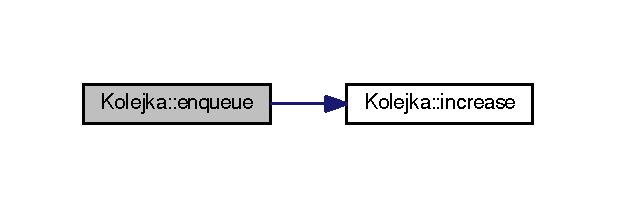
\includegraphics[width=296pt]{class_kolejka_a8f3b0111e85f517d9eadb8ce996d4471_cgraph}
\end{center}
\end{figure}




Here is the caller graph for this function\-:\nopagebreak
\begin{figure}[H]
\begin{center}
\leavevmode
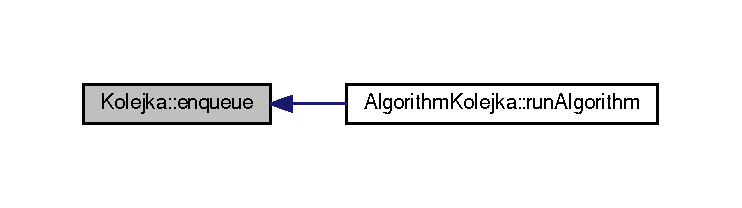
\includegraphics[width=350pt]{class_kolejka_a8f3b0111e85f517d9eadb8ce996d4471_icgraph}
\end{center}
\end{figure}


\hypertarget{class_kolejka_ab4f51f0ec7fef36a85af6cfd1c257427}{\index{Kolejka@{Kolejka}!increase@{increase}}
\index{increase@{increase}!Kolejka@{Kolejka}}
\subsubsection[{increase}]{\setlength{\rightskip}{0pt plus 5cm}void Kolejka\-::increase (
\begin{DoxyParamCaption}
{}
\end{DoxyParamCaption}
)\hspace{0.3cm}{\ttfamily [private]}}}\label{class_kolejka_ab4f51f0ec7fef36a85af6cfd1c257427}


Definition at line 27 of file kolejka.\-cpp.



Here is the caller graph for this function\-:\nopagebreak
\begin{figure}[H]
\begin{center}
\leavevmode
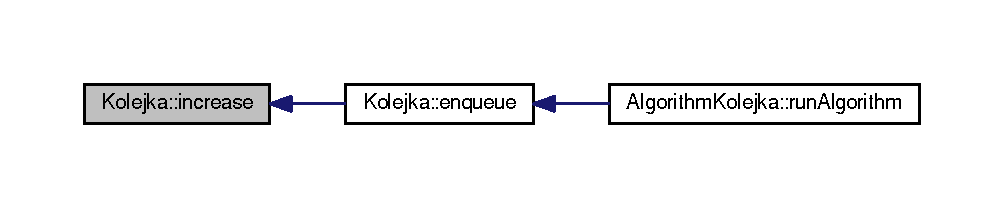
\includegraphics[width=350pt]{class_kolejka_ab4f51f0ec7fef36a85af6cfd1c257427_icgraph}
\end{center}
\end{figure}




\subsection{Member Data Documentation}
\hypertarget{class_kolejka_ae66597dc9eb1fcc210b075f8aa7ff77f}{\index{Kolejka@{Kolejka}!f@{f}}
\index{f@{f}!Kolejka@{Kolejka}}
\subsubsection[{f}]{\setlength{\rightskip}{0pt plus 5cm}int Kolejka\-::f\hspace{0.3cm}{\ttfamily [private]}}}\label{class_kolejka_ae66597dc9eb1fcc210b075f8aa7ff77f}


Definition at line 22 of file kolejka.\-hh.

\hypertarget{class_kolejka_ae16213a5b751800eb48da6bede435ad0}{\index{Kolejka@{Kolejka}!r@{r}}
\index{r@{r}!Kolejka@{Kolejka}}
\subsubsection[{r}]{\setlength{\rightskip}{0pt plus 5cm}int Kolejka\-::r\hspace{0.3cm}{\ttfamily [private]}}}\label{class_kolejka_ae16213a5b751800eb48da6bede435ad0}


Definition at line 26 of file kolejka.\-hh.

\hypertarget{class_kolejka_a84898848de8e77a76a6f2e4a7393b4bb}{\index{Kolejka@{Kolejka}!size@{size}}
\index{size@{size}!Kolejka@{Kolejka}}
\subsubsection[{size}]{\setlength{\rightskip}{0pt plus 5cm}long Kolejka\-::size\hspace{0.3cm}{\ttfamily [private]}}}\label{class_kolejka_a84898848de8e77a76a6f2e4a7393b4bb}


Definition at line 18 of file kolejka.\-hh.

\hypertarget{class_kolejka_a49e444e7bd7b91a78bc2a46426b73128}{\index{Kolejka@{Kolejka}!tab@{tab}}
\index{tab@{tab}!Kolejka@{Kolejka}}
\subsubsection[{tab}]{\setlength{\rightskip}{0pt plus 5cm}int$\ast$ Kolejka\-::tab\hspace{0.3cm}{\ttfamily [private]}}}\label{class_kolejka_a49e444e7bd7b91a78bc2a46426b73128}


Definition at line 14 of file kolejka.\-hh.



The documentation for this class was generated from the following files\-:\begin{DoxyCompactItemize}
\item 
\hyperlink{kolejka_8hh}{kolejka.\-hh}\item 
\hyperlink{kolejka_8cpp}{kolejka.\-cpp}\end{DoxyCompactItemize}

\hypertarget{struct_lista_1_1_komorka}{}\section{Lista\+:\+:Komorka Struct Reference}
\label{struct_lista_1_1_komorka}\index{Lista\+::\+Komorka@{Lista\+::\+Komorka}}


Struktura \hyperlink{struct_lista_1_1_komorka}{Komorka}. Obiekt tego typu reprezentuje pojedyncza komorke wraz ze wskaznikiem na nastepna komorke listy.  




Collaboration diagram for Lista\+:\+:Komorka\+:\nopagebreak
\begin{figure}[H]
\begin{center}
\leavevmode
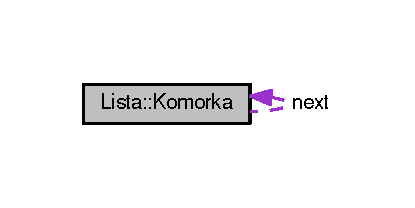
\includegraphics[width=199pt]{struct_lista_1_1_komorka__coll__graph}
\end{center}
\end{figure}
\subsection*{Public Member Functions}
\begin{DoxyCompactItemize}
\item 
\hyperlink{struct_lista_1_1_komorka_a1843c3c4ae9752cea90cfa21076f3e9c}{Komorka} (int \+\_\+elem)
\begin{DoxyCompactList}\small\item\em Konstruktor paramteryczny obiektu \hyperlink{struct_lista_1_1_komorka}{Komorka}. \end{DoxyCompactList}\end{DoxyCompactItemize}
\subsection*{Public Attributes}
\begin{DoxyCompactItemize}
\item 
int \hyperlink{struct_lista_1_1_komorka_aeb683e1dce8a8c096cc54a6645137411}{elem}
\begin{DoxyCompactList}\small\item\em Wartosc elementu w pojedynczej komorce. \end{DoxyCompactList}\item 
\hyperlink{struct_lista_1_1_komorka}{Komorka} $\ast$ \hyperlink{struct_lista_1_1_komorka_aa04e9d2ed0260f2adbff6855f7bcd77e}{next}
\begin{DoxyCompactList}\small\item\em Wskaznik na nastepna komorke listy. \end{DoxyCompactList}\end{DoxyCompactItemize}


\subsection{Detailed Description}


Definition at line 16 of file lista.\+hh.



\subsection{Constructor \& Destructor Documentation}
\hypertarget{struct_lista_1_1_komorka_a1843c3c4ae9752cea90cfa21076f3e9c}{}\index{Lista\+::\+Komorka@{Lista\+::\+Komorka}!Komorka@{Komorka}}
\index{Komorka@{Komorka}!Lista\+::\+Komorka@{Lista\+::\+Komorka}}
\subsubsection[{Komorka}]{\setlength{\rightskip}{0pt plus 5cm}Lista\+::\+Komorka\+::\+Komorka (
\begin{DoxyParamCaption}
\item[{int}]{\+\_\+elem}
\end{DoxyParamCaption}
)\hspace{0.3cm}{\ttfamily [inline]}}\label{struct_lista_1_1_komorka_a1843c3c4ae9752cea90cfa21076f3e9c}

\begin{DoxyParams}[1]{Parameters}
\mbox{\tt in}  & {\em \+\_\+elem} & -\/ wartosc przechowywanego elementu. \\
\hline
\end{DoxyParams}


Definition at line 29 of file lista.\+hh.



\subsection{Member Data Documentation}
\hypertarget{struct_lista_1_1_komorka_aeb683e1dce8a8c096cc54a6645137411}{}\index{Lista\+::\+Komorka@{Lista\+::\+Komorka}!elem@{elem}}
\index{elem@{elem}!Lista\+::\+Komorka@{Lista\+::\+Komorka}}
\subsubsection[{elem}]{\setlength{\rightskip}{0pt plus 5cm}int Lista\+::\+Komorka\+::elem}\label{struct_lista_1_1_komorka_aeb683e1dce8a8c096cc54a6645137411}


Definition at line 20 of file lista.\+hh.

\hypertarget{struct_lista_1_1_komorka_aa04e9d2ed0260f2adbff6855f7bcd77e}{}\index{Lista\+::\+Komorka@{Lista\+::\+Komorka}!next@{next}}
\index{next@{next}!Lista\+::\+Komorka@{Lista\+::\+Komorka}}
\subsubsection[{next}]{\setlength{\rightskip}{0pt plus 5cm}{\bf Komorka}$\ast$ Lista\+::\+Komorka\+::next}\label{struct_lista_1_1_komorka_aa04e9d2ed0260f2adbff6855f7bcd77e}


Definition at line 24 of file lista.\+hh.



The documentation for this struct was generated from the following file\+:\begin{DoxyCompactItemize}
\item 
\hyperlink{lista_8hh}{lista.\+hh}\end{DoxyCompactItemize}

\hypertarget{class_lista}{}\section{Lista Class Reference}
\label{class_lista}\index{Lista@{Lista}}


Klasa \hyperlink{class_lista}{Lista} modelujaca strukture danych typu lista. Obiekt tego typu reprezentuje strukture danych typu lista wraz z operacjami mozliwymi do wykonania na tej strukturze.  




{\ttfamily \#include $<$lista.\+hh$>$}



Collaboration diagram for Lista\+:\nopagebreak
\begin{figure}[H]
\begin{center}
\leavevmode
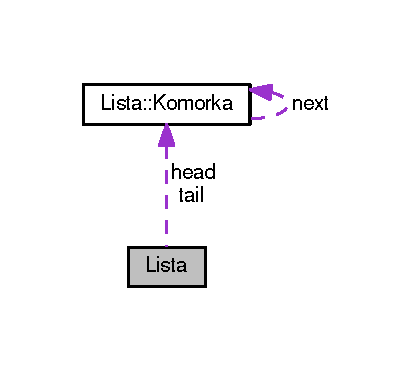
\includegraphics[width=199pt]{class_lista__coll__graph}
\end{center}
\end{figure}
\subsection*{Classes}
\begin{DoxyCompactItemize}
\item 
struct \hyperlink{struct_lista_1_1_komorka}{Komorka}
\begin{DoxyCompactList}\small\item\em Struktura \hyperlink{struct_lista_1_1_komorka}{Komorka}. Obiekt tego typu reprezentuje pojedyncza komorke wraz ze wskaznikiem na nastepna komorke listy. \end{DoxyCompactList}\end{DoxyCompactItemize}
\subsection*{Public Member Functions}
\begin{DoxyCompactItemize}
\item 
\hyperlink{class_lista_a1f668b36909182ef1360b48503529a31}{Lista} ()
\begin{DoxyCompactList}\small\item\em Konstruktor obiektu \hyperlink{class_lista}{Lista}. \end{DoxyCompactList}\item 
\hyperlink{class_lista_a4d7394b2728a00ad8404965b2e15d096}{$\sim$\+Lista} ()
\begin{DoxyCompactList}\small\item\em Destruktor obiektu \hyperlink{class_lista}{Lista}. \end{DoxyCompactList}\item 
void \hyperlink{class_lista_acec8ac807da644d8250c3c6043a208e1}{insert} (int \+\_\+elem)
\begin{DoxyCompactList}\small\item\em Metoda dodawnia elementu. Metoda sluzy do dodawania elementu do konca listy. \end{DoxyCompactList}\item 
int \hyperlink{class_lista_a18ce18bccb1af9b8d818f103021d7b4a}{remove} (int \+\_\+f)
\begin{DoxyCompactList}\small\item\em Metoda usuwania elementu. Metoda sluzy do usuwania elementu o wskazanym indeksie. \end{DoxyCompactList}\end{DoxyCompactItemize}
\subsection*{Private Attributes}
\begin{DoxyCompactItemize}
\item 
\hyperlink{struct_lista_1_1_komorka}{Komorka} $\ast$ \hyperlink{class_lista_aeba20505030183d334971bd44c3c8b95}{head}
\begin{DoxyCompactList}\small\item\em Wskaznik na poczatek listy. \end{DoxyCompactList}\item 
\hyperlink{struct_lista_1_1_komorka}{Komorka} $\ast$ \hyperlink{class_lista_a7d42e5f99e945d97c29d6f764f71f4e7}{tail}
\begin{DoxyCompactList}\small\item\em Wskaznik na koniec listy. \end{DoxyCompactList}\end{DoxyCompactItemize}


\subsection{Detailed Description}


Definition at line 9 of file lista.\+hh.



\subsection{Constructor \& Destructor Documentation}
\hypertarget{class_lista_a1f668b36909182ef1360b48503529a31}{}\index{Lista@{Lista}!Lista@{Lista}}
\index{Lista@{Lista}!Lista@{Lista}}
\subsubsection[{Lista}]{\setlength{\rightskip}{0pt plus 5cm}Lista\+::\+Lista (
\begin{DoxyParamCaption}
{}
\end{DoxyParamCaption}
)\hspace{0.3cm}{\ttfamily [inline]}}\label{class_lista_a1f668b36909182ef1360b48503529a31}


Definition at line 49 of file lista.\+hh.

\hypertarget{class_lista_a4d7394b2728a00ad8404965b2e15d096}{}\index{Lista@{Lista}!````~Lista@{$\sim$\+Lista}}
\index{````~Lista@{$\sim$\+Lista}!Lista@{Lista}}
\subsubsection[{$\sim$\+Lista}]{\setlength{\rightskip}{0pt plus 5cm}Lista\+::$\sim$\+Lista (
\begin{DoxyParamCaption}
{}
\end{DoxyParamCaption}
)\hspace{0.3cm}{\ttfamily [inline]}}\label{class_lista_a4d7394b2728a00ad8404965b2e15d096}


Definition at line 54 of file lista.\+hh.



\subsection{Member Function Documentation}
\hypertarget{class_lista_acec8ac807da644d8250c3c6043a208e1}{}\index{Lista@{Lista}!insert@{insert}}
\index{insert@{insert}!Lista@{Lista}}
\subsubsection[{insert}]{\setlength{\rightskip}{0pt plus 5cm}void Lista\+::insert (
\begin{DoxyParamCaption}
\item[{int}]{\+\_\+elem}
\end{DoxyParamCaption}
)}\label{class_lista_acec8ac807da644d8250c3c6043a208e1}

\begin{DoxyParams}[1]{Parameters}
\mbox{\tt in}  & {\em \+\_\+elem} & -\/ dodawany element. \\
\hline
\end{DoxyParams}


Definition at line 5 of file lista.\+cpp.



Here is the caller graph for this function\+:\nopagebreak
\begin{figure}[H]
\begin{center}
\leavevmode
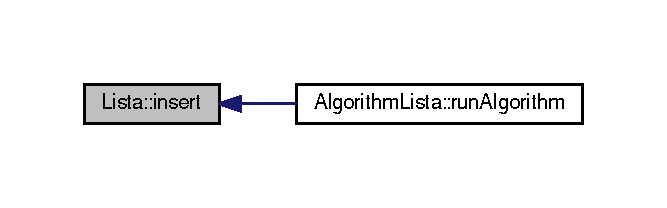
\includegraphics[width=320pt]{class_lista_acec8ac807da644d8250c3c6043a208e1_icgraph}
\end{center}
\end{figure}


\hypertarget{class_lista_a18ce18bccb1af9b8d818f103021d7b4a}{}\index{Lista@{Lista}!remove@{remove}}
\index{remove@{remove}!Lista@{Lista}}
\subsubsection[{remove}]{\setlength{\rightskip}{0pt plus 5cm}int Lista\+::remove (
\begin{DoxyParamCaption}
\item[{int}]{\+\_\+f}
\end{DoxyParamCaption}
)}\label{class_lista_a18ce18bccb1af9b8d818f103021d7b4a}

\begin{DoxyParams}[1]{Parameters}
\mbox{\tt in}  & {\em \+\_\+f} & -\/ indeks elementu do usuniecia. \\
\hline
\end{DoxyParams}
\begin{DoxyReturn}{Returns}
-\/ usuwany element. 
\end{DoxyReturn}


Definition at line 19 of file lista.\+cpp.



\subsection{Member Data Documentation}
\hypertarget{class_lista_aeba20505030183d334971bd44c3c8b95}{}\index{Lista@{Lista}!head@{head}}
\index{head@{head}!Lista@{Lista}}
\subsubsection[{head}]{\setlength{\rightskip}{0pt plus 5cm}{\bf Komorka}$\ast$ Lista\+::head\hspace{0.3cm}{\ttfamily [private]}}\label{class_lista_aeba20505030183d334971bd44c3c8b95}


Definition at line 38 of file lista.\+hh.

\hypertarget{class_lista_a7d42e5f99e945d97c29d6f764f71f4e7}{}\index{Lista@{Lista}!tail@{tail}}
\index{tail@{tail}!Lista@{Lista}}
\subsubsection[{tail}]{\setlength{\rightskip}{0pt plus 5cm}{\bf Komorka}$\ast$ Lista\+::tail\hspace{0.3cm}{\ttfamily [private]}}\label{class_lista_a7d42e5f99e945d97c29d6f764f71f4e7}


Definition at line 42 of file lista.\+hh.



The documentation for this class was generated from the following files\+:\begin{DoxyCompactItemize}
\item 
\hyperlink{lista_8hh}{lista.\+hh}\item 
\hyperlink{lista_8cpp}{lista.\+cpp}\end{DoxyCompactItemize}

\hypertarget{class_mnozenie}{\section{Mnozenie Class Reference}
\label{class_mnozenie}\index{Mnozenie@{Mnozenie}}
}


Klasa \hyperlink{class_mnozenie}{Mnozenie} modelujaca algorytm mnozenia. Obiekt tego typu reprezentuje algorytm wykonujacy dzialanie mnozenia kazdego elementu tablicy tab przez 2.  




{\ttfamily \#include $<$algorithm1.\-hh$>$}



Inheritance diagram for Mnozenie\-:\nopagebreak
\begin{figure}[H]
\begin{center}
\leavevmode
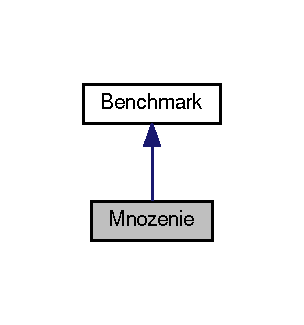
\includegraphics[width=146pt]{class_mnozenie__inherit__graph}
\end{center}
\end{figure}


Collaboration diagram for Mnozenie\-:\nopagebreak
\begin{figure}[H]
\begin{center}
\leavevmode
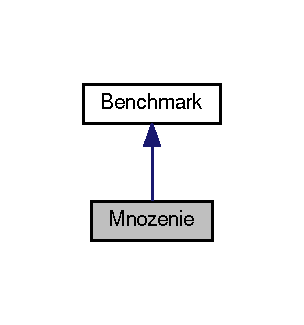
\includegraphics[width=146pt]{class_mnozenie__coll__graph}
\end{center}
\end{figure}
\subsection*{Public Member Functions}
\begin{DoxyCompactItemize}
\item 
\hyperlink{class_mnozenie_aac38391baa7ffd14970526902ab750de}{Mnozenie} ()
\begin{DoxyCompactList}\small\item\em Konstruktor obiektu \hyperlink{class_mnozenie}{Mnozenie}. \end{DoxyCompactList}\item 
\hyperlink{class_mnozenie_a8babd869ba0bd289e1e4287d6d8b56f2}{Mnozenie} (int \-\_\-tab\mbox{[}$\,$\mbox{]})
\begin{DoxyCompactList}\small\item\em Konstruktor parametryczny obiektu \hyperlink{class_mnozenie}{Mnozenie}. \end{DoxyCompactList}\item 
\hyperlink{class_mnozenie_ad57f03bc66770fb6a442169781ee2156}{$\sim$\-Mnozenie} ()
\begin{DoxyCompactList}\small\item\em Destruktor obiektu \hyperlink{class_mnozenie}{Mnozenie}. \end{DoxyCompactList}\item 
virtual void \hyperlink{class_mnozenie_a039792aaa5ce9723cd61d29869cf0101}{test\-Algorithm} (\hyperlink{class_benchmark}{Benchmark} $\ast$\-\_\-algorithm)
\begin{DoxyCompactList}\small\item\em Metoda testowania algorytmu. Metoda sluzy do testowania szybkosci dzialania algorytmu. W klasie \hyperlink{class_mnozenie}{Mnozenie} nie ma konkretnego dzialania. \end{DoxyCompactList}\item 
virtual void \hyperlink{class_mnozenie_a46b1c55b7ba208fa137065147e107be9}{run\-Algorithm} (int \-\_\-border)
\begin{DoxyCompactList}\small\item\em Metoda uruchamiania algorytmu. Metoda sluzy to wykonywania danego algorytmu. Mnozy kazdy element tablicy przez liczbe 2. \end{DoxyCompactList}\end{DoxyCompactItemize}
\subsection*{Private Attributes}
\begin{DoxyCompactItemize}
\item 
int \hyperlink{class_mnozenie_a6dc67671f84a557d97c322b8af528359}{tab} \mbox{[}\hyperlink{benchmark_8hh_a70ed59adcb4159ac551058053e649640}{S\-I\-Z\-E}\mbox{]}
\begin{DoxyCompactList}\small\item\em Tablica elementow z danymi wejsciowymi. \end{DoxyCompactList}\end{DoxyCompactItemize}


\subsection{Detailed Description}


Definition at line 9 of file algorithm1.\-hh.



\subsection{Constructor \& Destructor Documentation}
\hypertarget{class_mnozenie_aac38391baa7ffd14970526902ab750de}{\index{Mnozenie@{Mnozenie}!Mnozenie@{Mnozenie}}
\index{Mnozenie@{Mnozenie}!Mnozenie@{Mnozenie}}
\subsubsection[{Mnozenie}]{\setlength{\rightskip}{0pt plus 5cm}Mnozenie\-::\-Mnozenie (
\begin{DoxyParamCaption}
{}
\end{DoxyParamCaption}
)\hspace{0.3cm}{\ttfamily [inline]}}}\label{class_mnozenie_aac38391baa7ffd14970526902ab750de}


Definition at line 20 of file algorithm1.\-hh.

\hypertarget{class_mnozenie_a8babd869ba0bd289e1e4287d6d8b56f2}{\index{Mnozenie@{Mnozenie}!Mnozenie@{Mnozenie}}
\index{Mnozenie@{Mnozenie}!Mnozenie@{Mnozenie}}
\subsubsection[{Mnozenie}]{\setlength{\rightskip}{0pt plus 5cm}Mnozenie\-::\-Mnozenie (
\begin{DoxyParamCaption}
\item[{int}]{\-\_\-tab\mbox{[}$\,$\mbox{]}}
\end{DoxyParamCaption}
)\hspace{0.3cm}{\ttfamily [inline]}}}\label{class_mnozenie_a8babd869ba0bd289e1e4287d6d8b56f2}

\begin{DoxyParams}[1]{Parameters}
\mbox{\tt in}  & {\em \-\_\-tab} & -\/ tablica przechowujaca dane wejsciowe. \\
\hline
\end{DoxyParams}


Definition at line 26 of file algorithm1.\-hh.

\hypertarget{class_mnozenie_ad57f03bc66770fb6a442169781ee2156}{\index{Mnozenie@{Mnozenie}!$\sim$\-Mnozenie@{$\sim$\-Mnozenie}}
\index{$\sim$\-Mnozenie@{$\sim$\-Mnozenie}!Mnozenie@{Mnozenie}}
\subsubsection[{$\sim$\-Mnozenie}]{\setlength{\rightskip}{0pt plus 5cm}Mnozenie\-::$\sim$\-Mnozenie (
\begin{DoxyParamCaption}
{}
\end{DoxyParamCaption}
)\hspace{0.3cm}{\ttfamily [inline]}}}\label{class_mnozenie_ad57f03bc66770fb6a442169781ee2156}


Definition at line 31 of file algorithm1.\-hh.



\subsection{Member Function Documentation}
\hypertarget{class_mnozenie_a46b1c55b7ba208fa137065147e107be9}{\index{Mnozenie@{Mnozenie}!run\-Algorithm@{run\-Algorithm}}
\index{run\-Algorithm@{run\-Algorithm}!Mnozenie@{Mnozenie}}
\subsubsection[{run\-Algorithm}]{\setlength{\rightskip}{0pt plus 5cm}void Mnozenie\-::run\-Algorithm (
\begin{DoxyParamCaption}
\item[{int}]{\-\_\-border}
\end{DoxyParamCaption}
)\hspace{0.3cm}{\ttfamily [virtual]}}}\label{class_mnozenie_a46b1c55b7ba208fa137065147e107be9}

\begin{DoxyParams}[1]{Parameters}
\mbox{\tt in}  & {\em \-\_\-border} & -\/ ilosc elementow dla ktorych algorytm ma wykonac swoje dzialanie. \\
\hline
\end{DoxyParams}


Reimplemented from \hyperlink{class_benchmark_a6363894c058e8bfe146de09d7126b29c}{Benchmark}.



Definition at line 7 of file algorithm1.\-cpp.

\hypertarget{class_mnozenie_a039792aaa5ce9723cd61d29869cf0101}{\index{Mnozenie@{Mnozenie}!test\-Algorithm@{test\-Algorithm}}
\index{test\-Algorithm@{test\-Algorithm}!Mnozenie@{Mnozenie}}
\subsubsection[{test\-Algorithm}]{\setlength{\rightskip}{0pt plus 5cm}virtual void Mnozenie\-::test\-Algorithm (
\begin{DoxyParamCaption}
\item[{{\bf Benchmark} $\ast$}]{\-\_\-algorithm}
\end{DoxyParamCaption}
)\hspace{0.3cm}{\ttfamily [inline]}, {\ttfamily [virtual]}}}\label{class_mnozenie_a039792aaa5ce9723cd61d29869cf0101}

\begin{DoxyParams}[1]{Parameters}
\mbox{\tt in}  & {\em \-\_\-algorithm} & -\/ testowany algorytm. \\
\hline
\end{DoxyParams}


Definition at line 39 of file algorithm1.\-hh.



\subsection{Member Data Documentation}
\hypertarget{class_mnozenie_a6dc67671f84a557d97c322b8af528359}{\index{Mnozenie@{Mnozenie}!tab@{tab}}
\index{tab@{tab}!Mnozenie@{Mnozenie}}
\subsubsection[{tab}]{\setlength{\rightskip}{0pt plus 5cm}int Mnozenie\-::tab\mbox{[}{\bf S\-I\-Z\-E}\mbox{]}\hspace{0.3cm}{\ttfamily [private]}}}\label{class_mnozenie_a6dc67671f84a557d97c322b8af528359}


Definition at line 14 of file algorithm1.\-hh.



The documentation for this class was generated from the following files\-:\begin{DoxyCompactItemize}
\item 
\hyperlink{algorithm1_8hh}{algorithm1.\-hh}\item 
\hyperlink{algorithm1_8cpp}{algorithm1.\-cpp}\end{DoxyCompactItemize}

\hypertarget{class_stos}{\section{Stos Class Reference}
\label{class_stos}\index{Stos@{Stos}}
}


Klasa \hyperlink{class_stos}{Stos} modelujaca strukture danych typu stos. Obiekt tego typu reprezentuje strukture danych typu stos wraz z operacjami mozliwymi do wykonania na tej strukturze.  




{\ttfamily \#include $<$stos.\-hh$>$}

\subsection*{Public Member Functions}
\begin{DoxyCompactItemize}
\item 
\hyperlink{class_stos_a1de3b50386d5dfb56ddece17d0ea2389}{Stos} ()
\begin{DoxyCompactList}\small\item\em Konstruktor obiektu \hyperlink{class_stos}{Stos}. \end{DoxyCompactList}\item 
\hyperlink{class_stos_a6606affc11eed2b059b8caf287ffca25}{Stos} (long \-\_\-size)
\begin{DoxyCompactList}\small\item\em Konstruktor parametryczny obiektu \hyperlink{class_stos}{Stos}. \end{DoxyCompactList}\item 
\hyperlink{class_stos_af9a198e2540e18adcc0b5259105fd78e}{$\sim$\-Stos} ()
\begin{DoxyCompactList}\small\item\em Destruktor obiektu \hyperlink{class_stos}{Stos}. \end{DoxyCompactList}\item 
void \hyperlink{class_stos_afd5802e405946328cccca3eed676b493}{push} (int \-\_\-elem)
\begin{DoxyCompactList}\small\item\em Metoda dodawnia elementu. Metoda sluzy do dodawania elementu do stosu. \end{DoxyCompactList}\item 
int \hyperlink{class_stos_aabb14b8a389c55da6e2b50fbb179ed56}{pop} ()
\begin{DoxyCompactList}\small\item\em Metoda usuwania elementu. Metoda sluzy do usuwania elementu ze stosu. \end{DoxyCompactList}\end{DoxyCompactItemize}
\subsection*{Private Member Functions}
\begin{DoxyCompactItemize}
\item 
void \hyperlink{class_stos_aaf6e4717d1983c5351c9f5e9797368d3}{increase} ()
\begin{DoxyCompactList}\small\item\em Metoda powiekszania stosu. Metoda ta dodaje do stosu 8 kolejnych wolnych pol. \end{DoxyCompactList}\item 
int \hyperlink{class_stos_a1054dda0231b2516b6a04298801c0b27}{decrease} ()
\begin{DoxyCompactList}\small\item\em Metoda pomniejszania stosu. Metoda ta odejmuje od stosu jedno pole. \end{DoxyCompactList}\end{DoxyCompactItemize}
\subsection*{Private Attributes}
\begin{DoxyCompactItemize}
\item 
int $\ast$ \hyperlink{class_stos_abcb666dd5a69fe50228595dc8ac4160a}{tab}
\begin{DoxyCompactList}\small\item\em Wskaznik na tablice elementow stosu. \end{DoxyCompactList}\item 
long \hyperlink{class_stos_a07ba18a24f8f0dbd9144406d15bcd342}{size}
\begin{DoxyCompactList}\small\item\em Rozmiar stosu. \end{DoxyCompactList}\item 
long \hyperlink{class_stos_ae0623cdf9b6725e38da86b74972d61ba}{last}
\begin{DoxyCompactList}\small\item\em Indeks ostatniego wolnego pola. \end{DoxyCompactList}\end{DoxyCompactItemize}


\subsection{Detailed Description}


Definition at line 9 of file stos.\-hh.



\subsection{Constructor \& Destructor Documentation}
\hypertarget{class_stos_a1de3b50386d5dfb56ddece17d0ea2389}{\index{Stos@{Stos}!Stos@{Stos}}
\index{Stos@{Stos}!Stos@{Stos}}
\subsubsection[{Stos}]{\setlength{\rightskip}{0pt plus 5cm}Stos\-::\-Stos (
\begin{DoxyParamCaption}
{}
\end{DoxyParamCaption}
)}}\label{class_stos_a1de3b50386d5dfb56ddece17d0ea2389}


Definition at line 5 of file stos.\-cpp.

\hypertarget{class_stos_a6606affc11eed2b059b8caf287ffca25}{\index{Stos@{Stos}!Stos@{Stos}}
\index{Stos@{Stos}!Stos@{Stos}}
\subsubsection[{Stos}]{\setlength{\rightskip}{0pt plus 5cm}Stos\-::\-Stos (
\begin{DoxyParamCaption}
\item[{long}]{\-\_\-size}
\end{DoxyParamCaption}
)}}\label{class_stos_a6606affc11eed2b059b8caf287ffca25}

\begin{DoxyParams}[1]{Parameters}
\mbox{\tt in}  & {\em \-\_\-size} & -\/ rozmiar tworzonego stosu. \\
\hline
\end{DoxyParams}


Definition at line 14 of file stos.\-cpp.

\hypertarget{class_stos_af9a198e2540e18adcc0b5259105fd78e}{\index{Stos@{Stos}!$\sim$\-Stos@{$\sim$\-Stos}}
\index{$\sim$\-Stos@{$\sim$\-Stos}!Stos@{Stos}}
\subsubsection[{$\sim$\-Stos}]{\setlength{\rightskip}{0pt plus 5cm}Stos\-::$\sim$\-Stos (
\begin{DoxyParamCaption}
{}
\end{DoxyParamCaption}
)}}\label{class_stos_af9a198e2540e18adcc0b5259105fd78e}


Definition at line 23 of file stos.\-cpp.



\subsection{Member Function Documentation}
\hypertarget{class_stos_a1054dda0231b2516b6a04298801c0b27}{\index{Stos@{Stos}!decrease@{decrease}}
\index{decrease@{decrease}!Stos@{Stos}}
\subsubsection[{decrease}]{\setlength{\rightskip}{0pt plus 5cm}int Stos\-::decrease (
\begin{DoxyParamCaption}
{}
\end{DoxyParamCaption}
)\hspace{0.3cm}{\ttfamily [private]}}}\label{class_stos_a1054dda0231b2516b6a04298801c0b27}


Definition at line 53 of file stos.\-cpp.



Here is the caller graph for this function\-:\nopagebreak
\begin{figure}[H]
\begin{center}
\leavevmode
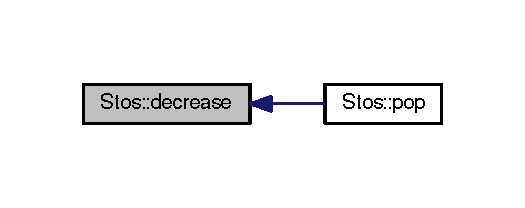
\includegraphics[width=256pt]{class_stos_a1054dda0231b2516b6a04298801c0b27_icgraph}
\end{center}
\end{figure}


\hypertarget{class_stos_aaf6e4717d1983c5351c9f5e9797368d3}{\index{Stos@{Stos}!increase@{increase}}
\index{increase@{increase}!Stos@{Stos}}
\subsubsection[{increase}]{\setlength{\rightskip}{0pt plus 5cm}void Stos\-::increase (
\begin{DoxyParamCaption}
{}
\end{DoxyParamCaption}
)\hspace{0.3cm}{\ttfamily [private]}}}\label{class_stos_aaf6e4717d1983c5351c9f5e9797368d3}


Definition at line 42 of file stos.\-cpp.



Here is the caller graph for this function\-:\nopagebreak
\begin{figure}[H]
\begin{center}
\leavevmode
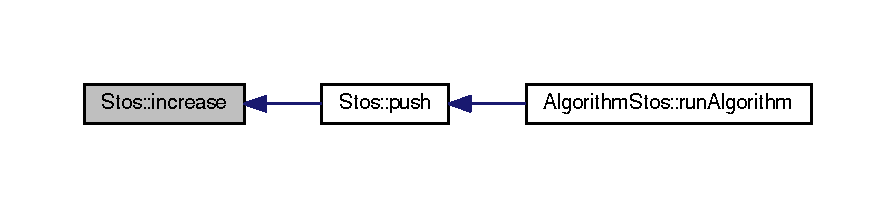
\includegraphics[width=350pt]{class_stos_aaf6e4717d1983c5351c9f5e9797368d3_icgraph}
\end{center}
\end{figure}


\hypertarget{class_stos_aabb14b8a389c55da6e2b50fbb179ed56}{\index{Stos@{Stos}!pop@{pop}}
\index{pop@{pop}!Stos@{Stos}}
\subsubsection[{pop}]{\setlength{\rightskip}{0pt plus 5cm}int Stos\-::pop (
\begin{DoxyParamCaption}
{}
\end{DoxyParamCaption}
)}}\label{class_stos_aabb14b8a389c55da6e2b50fbb179ed56}
\begin{DoxyReturn}{Returns}
-\/ usuwany element. 
\end{DoxyReturn}


Definition at line 35 of file stos.\-cpp.



Here is the call graph for this function\-:\nopagebreak
\begin{figure}[H]
\begin{center}
\leavevmode
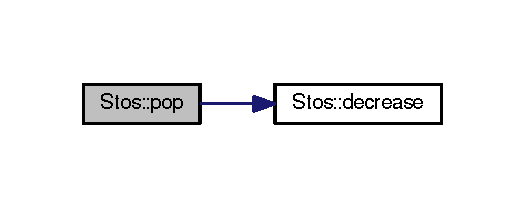
\includegraphics[width=256pt]{class_stos_aabb14b8a389c55da6e2b50fbb179ed56_cgraph}
\end{center}
\end{figure}


\hypertarget{class_stos_afd5802e405946328cccca3eed676b493}{\index{Stos@{Stos}!push@{push}}
\index{push@{push}!Stos@{Stos}}
\subsubsection[{push}]{\setlength{\rightskip}{0pt plus 5cm}void Stos\-::push (
\begin{DoxyParamCaption}
\item[{int}]{\-\_\-elem}
\end{DoxyParamCaption}
)}}\label{class_stos_afd5802e405946328cccca3eed676b493}

\begin{DoxyParams}[1]{Parameters}
\mbox{\tt in}  & {\em \-\_\-elem} & -\/ dodawany element. \\
\hline
\end{DoxyParams}


Definition at line 27 of file stos.\-cpp.



Here is the call graph for this function\-:\nopagebreak
\begin{figure}[H]
\begin{center}
\leavevmode
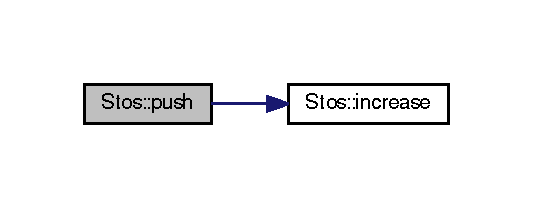
\includegraphics[width=256pt]{class_stos_afd5802e405946328cccca3eed676b493_cgraph}
\end{center}
\end{figure}




Here is the caller graph for this function\-:\nopagebreak
\begin{figure}[H]
\begin{center}
\leavevmode
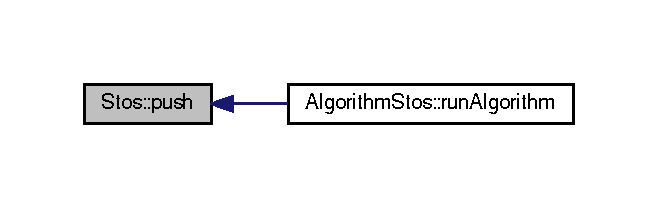
\includegraphics[width=316pt]{class_stos_afd5802e405946328cccca3eed676b493_icgraph}
\end{center}
\end{figure}




\subsection{Member Data Documentation}
\hypertarget{class_stos_ae0623cdf9b6725e38da86b74972d61ba}{\index{Stos@{Stos}!last@{last}}
\index{last@{last}!Stos@{Stos}}
\subsubsection[{last}]{\setlength{\rightskip}{0pt plus 5cm}long Stos\-::last\hspace{0.3cm}{\ttfamily [private]}}}\label{class_stos_ae0623cdf9b6725e38da86b74972d61ba}


Definition at line 22 of file stos.\-hh.

\hypertarget{class_stos_a07ba18a24f8f0dbd9144406d15bcd342}{\index{Stos@{Stos}!size@{size}}
\index{size@{size}!Stos@{Stos}}
\subsubsection[{size}]{\setlength{\rightskip}{0pt plus 5cm}long Stos\-::size\hspace{0.3cm}{\ttfamily [private]}}}\label{class_stos_a07ba18a24f8f0dbd9144406d15bcd342}


Definition at line 18 of file stos.\-hh.

\hypertarget{class_stos_abcb666dd5a69fe50228595dc8ac4160a}{\index{Stos@{Stos}!tab@{tab}}
\index{tab@{tab}!Stos@{Stos}}
\subsubsection[{tab}]{\setlength{\rightskip}{0pt plus 5cm}int$\ast$ Stos\-::tab\hspace{0.3cm}{\ttfamily [private]}}}\label{class_stos_abcb666dd5a69fe50228595dc8ac4160a}


Definition at line 14 of file stos.\-hh.



The documentation for this class was generated from the following files\-:\begin{DoxyCompactItemize}
\item 
\hyperlink{stos_8hh}{stos.\-hh}\item 
\hyperlink{stos_8cpp}{stos.\-cpp}\end{DoxyCompactItemize}

\hypertarget{class_tab_lista}{\section{Tab\-Lista Class Reference}
\label{class_tab_lista}\index{Tab\-Lista@{Tab\-Lista}}
}


Klasa \hyperlink{class_tab_lista}{Tab\-Lista} modelujaca strukture danych typu lista. Obiekt tego typu reprezentuje strukture danych typu lista zaimplementowana na tablicy dynamicznej. Obiekt zawiera rowniez podstowe metody listy.  




{\ttfamily \#include $<$tab\-\_\-lista.\-hh$>$}

\subsection*{Public Member Functions}
\begin{DoxyCompactItemize}
\item 
\hyperlink{class_tab_lista_ad3bfa98306e98b4e5bb7ff524e72078c}{Tab\-Lista} ()
\begin{DoxyCompactList}\small\item\em Konstruktor obiektu \hyperlink{class_tab_lista}{Tab\-Lista}. \end{DoxyCompactList}\item 
\hyperlink{class_tab_lista_a95d23d52e0af187351b3fc1022ae4839}{Tab\-Lista} (long \-\_\-size)
\begin{DoxyCompactList}\small\item\em Konstruktor parametryczny obiektu \hyperlink{class_tab_lista}{Tab\-Lista}. \end{DoxyCompactList}\item 
\hyperlink{class_tab_lista_a0b4a808158b370bbc5785ceef760a273}{$\sim$\-Tab\-Lista} ()
\begin{DoxyCompactList}\small\item\em Destruktor obiektu \hyperlink{class_tab_lista}{Tab\-Lista}. \end{DoxyCompactList}\item 
void \hyperlink{class_tab_lista_a7bd3e5f62a81bfd3813ad874e8a9c059}{insert} (int \-\_\-elem)
\begin{DoxyCompactList}\small\item\em Metoda dodawnia elementu. Metoda sluzy do dodawania elementu do konca listy. \end{DoxyCompactList}\item 
int \hyperlink{class_tab_lista_aae59a3eafbbd7424a952badb26410a5e}{remove} (int \-\_\-f)
\begin{DoxyCompactList}\small\item\em Metoda usuwania elementu. Metoda sluzy do usuwania elementu o wskazanym indeksie. \end{DoxyCompactList}\item 
int \hyperlink{class_tab_lista_ac4b9b266a861fc7ecffd60257a480991}{rozmiar} ()
\begin{DoxyCompactList}\small\item\em Metoda rozmiaru tablicy. Metoda zwraca ilosc elementow obecnych na tablicy. \end{DoxyCompactList}\item 
void \hyperlink{class_tab_lista_a7e7acd97b2675b82b9a0f50907e87c22}{quicksort} (int a, int b)
\begin{DoxyCompactList}\small\item\em Metoda sortujaca tablice. Metoda sluzy do sortowania tablicy. \end{DoxyCompactList}\end{DoxyCompactItemize}
\subsection*{Private Member Functions}
\begin{DoxyCompactItemize}
\item 
void \hyperlink{class_tab_lista_a9ae6a784d488c8b9885ccbc945225f9e}{increase} ()
\begin{DoxyCompactList}\small\item\em Metoda powiekszania listy tablicowe. Metoda ta dodaje do listy 8 kolejnych wolnych pol. \end{DoxyCompactList}\end{DoxyCompactItemize}
\subsection*{Private Attributes}
\begin{DoxyCompactItemize}
\item 
int $\ast$ \hyperlink{class_tab_lista_a06f658ed62f3db852813e90dcc5876a5}{tab}
\begin{DoxyCompactList}\small\item\em Wskaznik na tablice elementow listy. \end{DoxyCompactList}\item 
long \hyperlink{class_tab_lista_aa3c6d623be318ec8410fa447281380da}{size}
\begin{DoxyCompactList}\small\item\em Rozmiar listy. \end{DoxyCompactList}\item 
long \hyperlink{class_tab_lista_ac7413a3d41c2c2e57fa92e055fc2e5b3}{last}
\begin{DoxyCompactList}\small\item\em Wskaznik na ostatni wolny element. \end{DoxyCompactList}\end{DoxyCompactItemize}


\subsection{Detailed Description}


Definition at line 10 of file tab\-\_\-lista.\-hh.



\subsection{Constructor \& Destructor Documentation}
\hypertarget{class_tab_lista_ad3bfa98306e98b4e5bb7ff524e72078c}{\index{Tab\-Lista@{Tab\-Lista}!Tab\-Lista@{Tab\-Lista}}
\index{Tab\-Lista@{Tab\-Lista}!TabLista@{Tab\-Lista}}
\subsubsection[{Tab\-Lista}]{\setlength{\rightskip}{0pt plus 5cm}Tab\-Lista\-::\-Tab\-Lista (
\begin{DoxyParamCaption}
{}
\end{DoxyParamCaption}
)}}\label{class_tab_lista_ad3bfa98306e98b4e5bb7ff524e72078c}


Definition at line 5 of file tab\-\_\-lista.\-cpp.

\hypertarget{class_tab_lista_a95d23d52e0af187351b3fc1022ae4839}{\index{Tab\-Lista@{Tab\-Lista}!Tab\-Lista@{Tab\-Lista}}
\index{Tab\-Lista@{Tab\-Lista}!TabLista@{Tab\-Lista}}
\subsubsection[{Tab\-Lista}]{\setlength{\rightskip}{0pt plus 5cm}Tab\-Lista\-::\-Tab\-Lista (
\begin{DoxyParamCaption}
\item[{long}]{\-\_\-size}
\end{DoxyParamCaption}
)}}\label{class_tab_lista_a95d23d52e0af187351b3fc1022ae4839}


Definition at line 13 of file tab\-\_\-lista.\-cpp.

\hypertarget{class_tab_lista_a0b4a808158b370bbc5785ceef760a273}{\index{Tab\-Lista@{Tab\-Lista}!$\sim$\-Tab\-Lista@{$\sim$\-Tab\-Lista}}
\index{$\sim$\-Tab\-Lista@{$\sim$\-Tab\-Lista}!TabLista@{Tab\-Lista}}
\subsubsection[{$\sim$\-Tab\-Lista}]{\setlength{\rightskip}{0pt plus 5cm}Tab\-Lista\-::$\sim$\-Tab\-Lista (
\begin{DoxyParamCaption}
{}
\end{DoxyParamCaption}
)}}\label{class_tab_lista_a0b4a808158b370bbc5785ceef760a273}


Definition at line 21 of file tab\-\_\-lista.\-cpp.



\subsection{Member Function Documentation}
\hypertarget{class_tab_lista_a9ae6a784d488c8b9885ccbc945225f9e}{\index{Tab\-Lista@{Tab\-Lista}!increase@{increase}}
\index{increase@{increase}!TabLista@{Tab\-Lista}}
\subsubsection[{increase}]{\setlength{\rightskip}{0pt plus 5cm}void Tab\-Lista\-::increase (
\begin{DoxyParamCaption}
{}
\end{DoxyParamCaption}
)\hspace{0.3cm}{\ttfamily [private]}}}\label{class_tab_lista_a9ae6a784d488c8b9885ccbc945225f9e}


Definition at line 25 of file tab\-\_\-lista.\-cpp.



Here is the caller graph for this function\-:\nopagebreak
\begin{figure}[H]
\begin{center}
\leavevmode
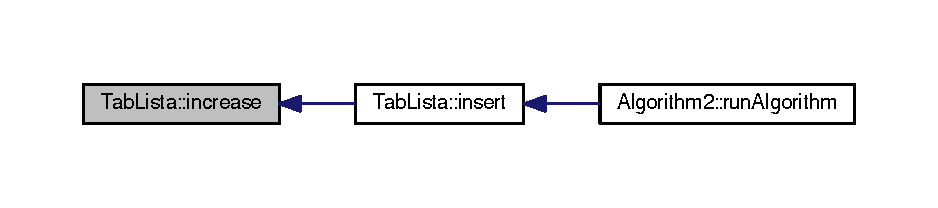
\includegraphics[width=350pt]{class_tab_lista_a9ae6a784d488c8b9885ccbc945225f9e_icgraph}
\end{center}
\end{figure}


\hypertarget{class_tab_lista_a7bd3e5f62a81bfd3813ad874e8a9c059}{\index{Tab\-Lista@{Tab\-Lista}!insert@{insert}}
\index{insert@{insert}!TabLista@{Tab\-Lista}}
\subsubsection[{insert}]{\setlength{\rightskip}{0pt plus 5cm}void Tab\-Lista\-::insert (
\begin{DoxyParamCaption}
\item[{int}]{\-\_\-elem}
\end{DoxyParamCaption}
)}}\label{class_tab_lista_a7bd3e5f62a81bfd3813ad874e8a9c059}

\begin{DoxyParams}[1]{Parameters}
\mbox{\tt in}  & {\em \-\_\-elem} & -\/ dodawany element. \\
\hline
\end{DoxyParams}


Definition at line 35 of file tab\-\_\-lista.\-cpp.



Here is the call graph for this function\-:\nopagebreak
\begin{figure}[H]
\begin{center}
\leavevmode
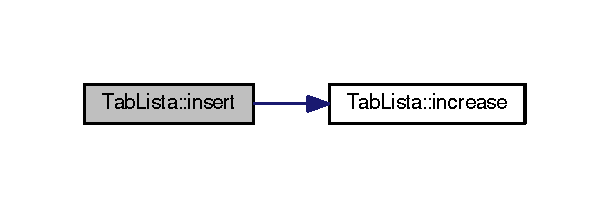
\includegraphics[width=296pt]{class_tab_lista_a7bd3e5f62a81bfd3813ad874e8a9c059_cgraph}
\end{center}
\end{figure}




Here is the caller graph for this function\-:\nopagebreak
\begin{figure}[H]
\begin{center}
\leavevmode
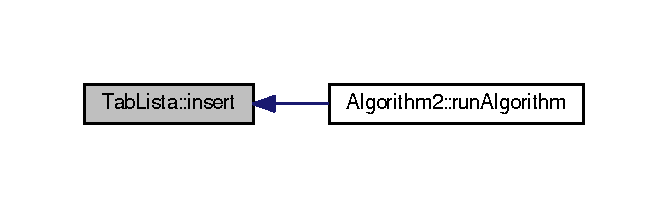
\includegraphics[width=322pt]{class_tab_lista_a7bd3e5f62a81bfd3813ad874e8a9c059_icgraph}
\end{center}
\end{figure}


\hypertarget{class_tab_lista_a7e7acd97b2675b82b9a0f50907e87c22}{\index{Tab\-Lista@{Tab\-Lista}!quicksort@{quicksort}}
\index{quicksort@{quicksort}!TabLista@{Tab\-Lista}}
\subsubsection[{quicksort}]{\setlength{\rightskip}{0pt plus 5cm}void Tab\-Lista\-::quicksort (
\begin{DoxyParamCaption}
\item[{int}]{a, }
\item[{int}]{b}
\end{DoxyParamCaption}
)}}\label{class_tab_lista_a7e7acd97b2675b82b9a0f50907e87c22}

\begin{DoxyParams}[1]{Parameters}
\mbox{\tt in}  & {\em a} & -\/ lewy zakres sortowania. \\
\hline
\mbox{\tt in}  & {\em b} & -\/ prawy zakres sortowania. \\
\hline
\end{DoxyParams}


Definition at line 57 of file tab\-\_\-lista.\-cpp.



Here is the caller graph for this function\-:\nopagebreak
\begin{figure}[H]
\begin{center}
\leavevmode
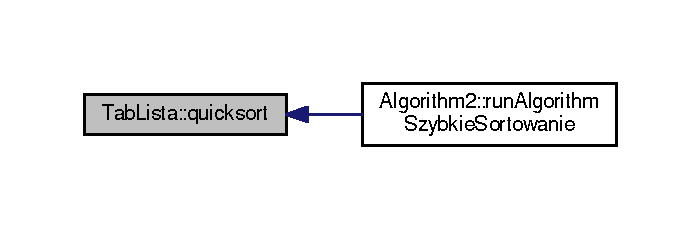
\includegraphics[width=336pt]{class_tab_lista_a7e7acd97b2675b82b9a0f50907e87c22_icgraph}
\end{center}
\end{figure}


\hypertarget{class_tab_lista_aae59a3eafbbd7424a952badb26410a5e}{\index{Tab\-Lista@{Tab\-Lista}!remove@{remove}}
\index{remove@{remove}!TabLista@{Tab\-Lista}}
\subsubsection[{remove}]{\setlength{\rightskip}{0pt plus 5cm}int Tab\-Lista\-::remove (
\begin{DoxyParamCaption}
\item[{int}]{\-\_\-f}
\end{DoxyParamCaption}
)}}\label{class_tab_lista_aae59a3eafbbd7424a952badb26410a5e}

\begin{DoxyParams}[1]{Parameters}
\mbox{\tt in}  & {\em \-\_\-f} & -\/ indeks elementu do usuniecia. \\
\hline
\end{DoxyParams}
\begin{DoxyReturn}{Returns}
-\/ usuwany element. 
\end{DoxyReturn}


Definition at line 42 of file tab\-\_\-lista.\-cpp.

\hypertarget{class_tab_lista_ac4b9b266a861fc7ecffd60257a480991}{\index{Tab\-Lista@{Tab\-Lista}!rozmiar@{rozmiar}}
\index{rozmiar@{rozmiar}!TabLista@{Tab\-Lista}}
\subsubsection[{rozmiar}]{\setlength{\rightskip}{0pt plus 5cm}int Tab\-Lista\-::rozmiar (
\begin{DoxyParamCaption}
{}
\end{DoxyParamCaption}
)}}\label{class_tab_lista_ac4b9b266a861fc7ecffd60257a480991}
\begin{DoxyReturn}{Returns}
-\/ ilosc elementow na tablicy. 
\end{DoxyReturn}


Definition at line 112 of file tab\-\_\-lista.\-cpp.



\subsection{Member Data Documentation}
\hypertarget{class_tab_lista_ac7413a3d41c2c2e57fa92e055fc2e5b3}{\index{Tab\-Lista@{Tab\-Lista}!last@{last}}
\index{last@{last}!TabLista@{Tab\-Lista}}
\subsubsection[{last}]{\setlength{\rightskip}{0pt plus 5cm}long Tab\-Lista\-::last\hspace{0.3cm}{\ttfamily [private]}}}\label{class_tab_lista_ac7413a3d41c2c2e57fa92e055fc2e5b3}


Definition at line 23 of file tab\-\_\-lista.\-hh.

\hypertarget{class_tab_lista_aa3c6d623be318ec8410fa447281380da}{\index{Tab\-Lista@{Tab\-Lista}!size@{size}}
\index{size@{size}!TabLista@{Tab\-Lista}}
\subsubsection[{size}]{\setlength{\rightskip}{0pt plus 5cm}long Tab\-Lista\-::size\hspace{0.3cm}{\ttfamily [private]}}}\label{class_tab_lista_aa3c6d623be318ec8410fa447281380da}


Definition at line 19 of file tab\-\_\-lista.\-hh.

\hypertarget{class_tab_lista_a06f658ed62f3db852813e90dcc5876a5}{\index{Tab\-Lista@{Tab\-Lista}!tab@{tab}}
\index{tab@{tab}!TabLista@{Tab\-Lista}}
\subsubsection[{tab}]{\setlength{\rightskip}{0pt plus 5cm}int$\ast$ Tab\-Lista\-::tab\hspace{0.3cm}{\ttfamily [private]}}}\label{class_tab_lista_a06f658ed62f3db852813e90dcc5876a5}


Definition at line 15 of file tab\-\_\-lista.\-hh.



The documentation for this class was generated from the following files\-:\begin{DoxyCompactItemize}
\item 
\hyperlink{tab__lista_8hh}{tab\-\_\-lista.\-hh}\item 
\hyperlink{tab__lista_8cpp}{tab\-\_\-lista.\-cpp}\end{DoxyCompactItemize}

\chapter{File Documentation}
\hypertarget{algorithm1_8cpp}{\section{algorithm1.\-cpp File Reference}
\label{algorithm1_8cpp}\index{algorithm1.\-cpp@{algorithm1.\-cpp}}
}
{\ttfamily \#include $<$iostream$>$}\\*
{\ttfamily \#include \char`\"{}benchmark.\-hh\char`\"{}}\\*
{\ttfamily \#include \char`\"{}algorithm1.\-hh\char`\"{}}\\*
Include dependency graph for algorithm1.\-cpp\-:\nopagebreak
\begin{figure}[H]
\begin{center}
\leavevmode
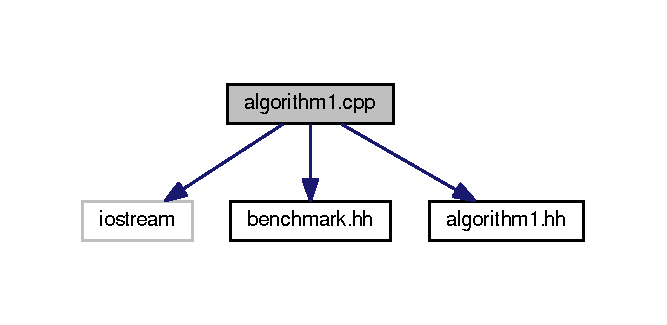
\includegraphics[width=322pt]{algorithm1_8cpp__incl}
\end{center}
\end{figure}

\hypertarget{algorithm1_8hh}{\section{algorithm1.\-hh File Reference}
\label{algorithm1_8hh}\index{algorithm1.\-hh@{algorithm1.\-hh}}
}
This graph shows which files directly or indirectly include this file\-:\nopagebreak
\begin{figure}[H]
\begin{center}
\leavevmode
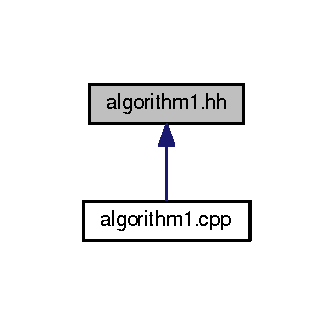
\includegraphics[width=160pt]{algorithm1_8hh__dep__incl}
\end{center}
\end{figure}
\subsection*{Classes}
\begin{DoxyCompactItemize}
\item 
class \hyperlink{class_mnozenie}{Mnozenie}
\begin{DoxyCompactList}\small\item\em Klasa \hyperlink{class_mnozenie}{Mnozenie} modelujaca algorytm mnozenia. Obiekt tego typu reprezentuje algorytm wykonujacy dzialanie mnozenia kazdego elementu tablicy tab przez 2. \end{DoxyCompactList}\end{DoxyCompactItemize}

\hypertarget{algorithm2_8cpp}{}\section{algorithm2.\+cpp File Reference}
\label{algorithm2_8cpp}\index{algorithm2.\+cpp@{algorithm2.\+cpp}}
{\ttfamily \#include $<$iostream$>$}\\*
{\ttfamily \#include \char`\"{}tab\+\_\+lista.\+hh\char`\"{}}\\*
{\ttfamily \#include \char`\"{}benchmark.\+hh\char`\"{}}\\*
{\ttfamily \#include \char`\"{}algorithm2.\+hh\char`\"{}}\\*
Include dependency graph for algorithm2.\+cpp\+:\nopagebreak
\begin{figure}[H]
\begin{center}
\leavevmode
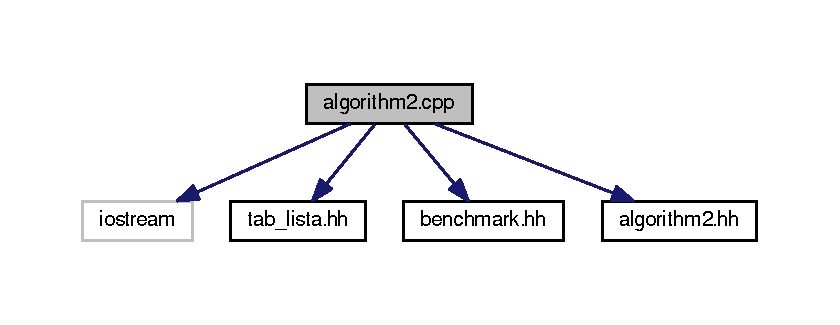
\includegraphics[width=350pt]{algorithm2_8cpp__incl}
\end{center}
\end{figure}

\hypertarget{algorithm2_8hh}{\section{algorithm2.\-hh File Reference}
\label{algorithm2_8hh}\index{algorithm2.\-hh@{algorithm2.\-hh}}
}
This graph shows which files directly or indirectly include this file\-:\nopagebreak
\begin{figure}[H]
\begin{center}
\leavevmode
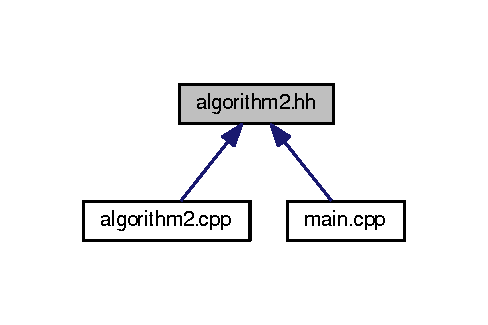
\includegraphics[width=234pt]{algorithm2_8hh__dep__incl}
\end{center}
\end{figure}
\subsection*{Classes}
\begin{DoxyCompactItemize}
\item 
class \hyperlink{class_algorithm2}{Algorithm2}
\begin{DoxyCompactList}\small\item\em Klasa \hyperlink{class_algorithm2}{Algorithm2} modelujaca algorytm wczytywania do listy tablicowej. Obiekt tego typu reprezentuje algorytm wykonujacy wykonujacy wczytywanie zadanej ilosci elementow do listy tablicowej. \end{DoxyCompactList}\end{DoxyCompactItemize}

\hypertarget{algorithm__kolejka_8cpp}{}\section{algorithm\+\_\+kolejka.\+cpp File Reference}
\label{algorithm__kolejka_8cpp}\index{algorithm\+\_\+kolejka.\+cpp@{algorithm\+\_\+kolejka.\+cpp}}
{\ttfamily \#include $<$iostream$>$}\\*
{\ttfamily \#include \char`\"{}kolejka.\+hh\char`\"{}}\\*
{\ttfamily \#include \char`\"{}benchmark.\+hh\char`\"{}}\\*
{\ttfamily \#include \char`\"{}algorithm\+\_\+kolejka.\+hh\char`\"{}}\\*
Include dependency graph for algorithm\+\_\+kolejka.\+cpp\+:\nopagebreak
\begin{figure}[H]
\begin{center}
\leavevmode
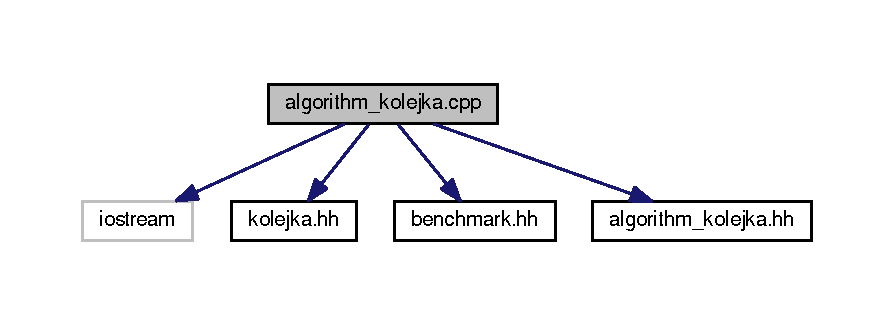
\includegraphics[width=350pt]{algorithm__kolejka_8cpp__incl}
\end{center}
\end{figure}

\hypertarget{algorithm__kolejka_8hh}{}\section{algorithm\+\_\+kolejka.\+hh File Reference}
\label{algorithm__kolejka_8hh}\index{algorithm\+\_\+kolejka.\+hh@{algorithm\+\_\+kolejka.\+hh}}
This graph shows which files directly or indirectly include this file\+:\nopagebreak
\begin{figure}[H]
\begin{center}
\leavevmode
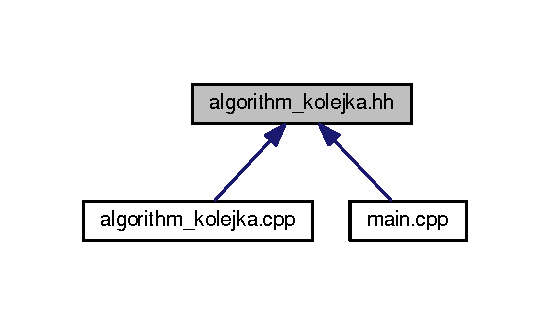
\includegraphics[width=264pt]{algorithm__kolejka_8hh__dep__incl}
\end{center}
\end{figure}
\subsection*{Classes}
\begin{DoxyCompactItemize}
\item 
class \hyperlink{class_algorithm_kolejka}{Algorithm\+Kolejka}
\begin{DoxyCompactList}\small\item\em Klasa \hyperlink{class_algorithm_kolejka}{Algorithm\+Kolejka} modelujaca algorytm wczytywania do kolejki. Obiekt tego typu reprezentuje algorytm wykonujacy wykonujacy wczytywanie zadanej ilosci elementow do kolejki. \end{DoxyCompactList}\end{DoxyCompactItemize}

\hypertarget{algorithm__lista_8cpp}{\section{algorithm\-\_\-lista.\-cpp File Reference}
\label{algorithm__lista_8cpp}\index{algorithm\-\_\-lista.\-cpp@{algorithm\-\_\-lista.\-cpp}}
}
{\ttfamily \#include $<$iostream$>$}\\*
{\ttfamily \#include \char`\"{}lista.\-hh\char`\"{}}\\*
{\ttfamily \#include \char`\"{}benchmark.\-hh\char`\"{}}\\*
{\ttfamily \#include \char`\"{}algorithm\-\_\-lista.\-hh\char`\"{}}\\*
Include dependency graph for algorithm\-\_\-lista.\-cpp\-:\nopagebreak
\begin{figure}[H]
\begin{center}
\leavevmode
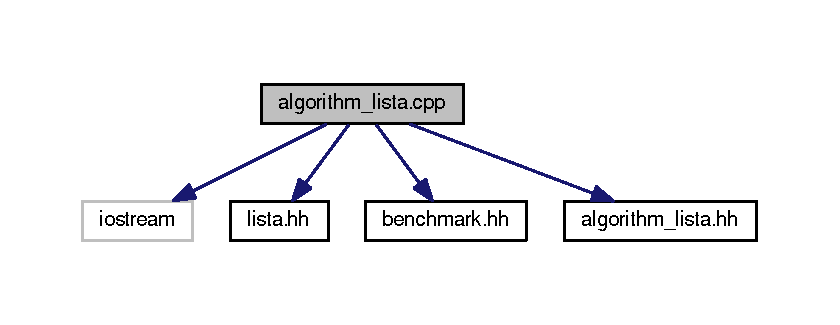
\includegraphics[width=350pt]{algorithm__lista_8cpp__incl}
\end{center}
\end{figure}

\hypertarget{algorithm__lista_8hh}{\section{algorithm\-\_\-lista.\-hh File Reference}
\label{algorithm__lista_8hh}\index{algorithm\-\_\-lista.\-hh@{algorithm\-\_\-lista.\-hh}}
}
This graph shows which files directly or indirectly include this file\-:\nopagebreak
\begin{figure}[H]
\begin{center}
\leavevmode
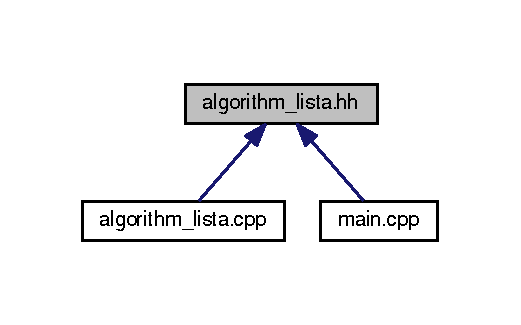
\includegraphics[width=252pt]{algorithm__lista_8hh__dep__incl}
\end{center}
\end{figure}
\subsection*{Classes}
\begin{DoxyCompactItemize}
\item 
class \hyperlink{class_algorithm_lista}{Algorithm\-Lista}
\begin{DoxyCompactList}\small\item\em Klasa \hyperlink{class_algorithm_lista}{Algorithm\-Lista} modelujaca algorytm wczytywania do kolejki. Obiekt tego typu reprezentuje algorytm wykonujacy wykonujacy wczytywanie zadanej ilosci elementow do listy. \end{DoxyCompactList}\end{DoxyCompactItemize}

\hypertarget{algorithm__stos_8cpp}{}\section{algorithm\+\_\+stos.\+cpp File Reference}
\label{algorithm__stos_8cpp}\index{algorithm\+\_\+stos.\+cpp@{algorithm\+\_\+stos.\+cpp}}
{\ttfamily \#include $<$iostream$>$}\\*
{\ttfamily \#include \char`\"{}stos.\+hh\char`\"{}}\\*
{\ttfamily \#include \char`\"{}benchmark.\+hh\char`\"{}}\\*
{\ttfamily \#include \char`\"{}algorithm\+\_\+stos.\+hh\char`\"{}}\\*
Include dependency graph for algorithm\+\_\+stos.\+cpp\+:\nopagebreak
\begin{figure}[H]
\begin{center}
\leavevmode
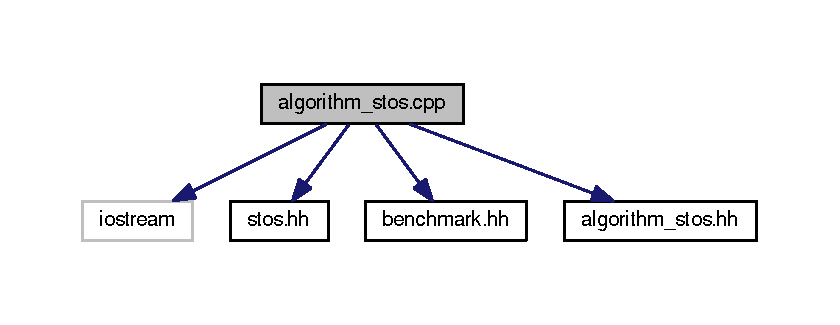
\includegraphics[width=350pt]{algorithm__stos_8cpp__incl}
\end{center}
\end{figure}

\hypertarget{algorithm__stos_8hh}{\section{algorithm\-\_\-stos.\-hh File Reference}
\label{algorithm__stos_8hh}\index{algorithm\-\_\-stos.\-hh@{algorithm\-\_\-stos.\-hh}}
}
This graph shows which files directly or indirectly include this file\-:\nopagebreak
\begin{figure}[H]
\begin{center}
\leavevmode
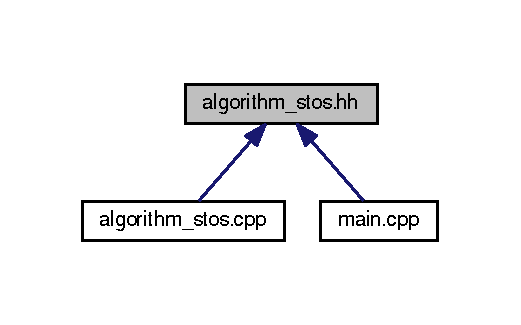
\includegraphics[width=252pt]{algorithm__stos_8hh__dep__incl}
\end{center}
\end{figure}
\subsection*{Classes}
\begin{DoxyCompactItemize}
\item 
class \hyperlink{class_algorithm_stos}{Algorithm\-Stos}
\begin{DoxyCompactList}\small\item\em Klasa \hyperlink{class_algorithm_stos}{Algorithm\-Stos} modelujaca algorytm wczytywania do stosu. Obiekt tego typu reprezentuje algorytm wykonujacy wykonujacy wczytywanie zadanej ilosci elementow do stosu. \end{DoxyCompactList}\end{DoxyCompactItemize}

\hypertarget{benchmark_8cpp}{}\section{benchmark.\+cpp File Reference}
\label{benchmark_8cpp}\index{benchmark.\+cpp@{benchmark.\+cpp}}
{\ttfamily \#include $<$iostream$>$}\\*
{\ttfamily \#include $<$fstream$>$}\\*
{\ttfamily \#include $<$chrono$>$}\\*
{\ttfamily \#include \char`\"{}benchmark.\+hh\char`\"{}}\\*
Include dependency graph for benchmark.\+cpp\+:\nopagebreak
\begin{figure}[H]
\begin{center}
\leavevmode
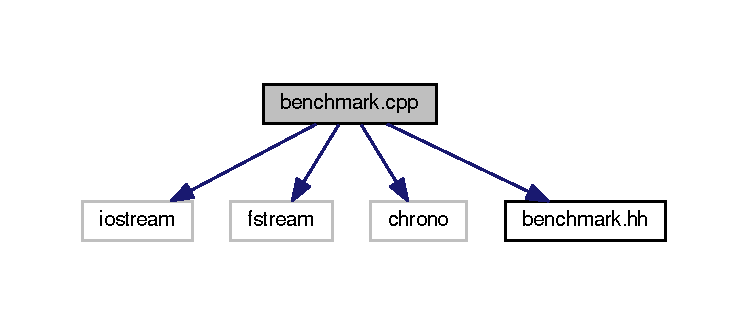
\includegraphics[width=350pt]{benchmark_8cpp__incl}
\end{center}
\end{figure}
\subsection*{Macros}
\begin{DoxyCompactItemize}
\item 
\#define \hyperlink{benchmark_8cpp_a30362161c93e3f1a4ee4c673f535b5a8}{L\+E\+N\+G\+T\+H}~100
\item 
\#define \hyperlink{benchmark_8cpp_a96de703b1d261e201a5cbb65b4590f89}{R\+E\+P\+E\+A\+T\+S}~4
\end{DoxyCompactItemize}


\subsection{Macro Definition Documentation}
\hypertarget{benchmark_8cpp_a30362161c93e3f1a4ee4c673f535b5a8}{}\index{benchmark.\+cpp@{benchmark.\+cpp}!L\+E\+N\+G\+T\+H@{L\+E\+N\+G\+T\+H}}
\index{L\+E\+N\+G\+T\+H@{L\+E\+N\+G\+T\+H}!benchmark.\+cpp@{benchmark.\+cpp}}
\subsubsection[{L\+E\+N\+G\+T\+H}]{\setlength{\rightskip}{0pt plus 5cm}\#define L\+E\+N\+G\+T\+H~100}\label{benchmark_8cpp_a30362161c93e3f1a4ee4c673f535b5a8}


Definition at line 7 of file benchmark.\+cpp.

\hypertarget{benchmark_8cpp_a96de703b1d261e201a5cbb65b4590f89}{}\index{benchmark.\+cpp@{benchmark.\+cpp}!R\+E\+P\+E\+A\+T\+S@{R\+E\+P\+E\+A\+T\+S}}
\index{R\+E\+P\+E\+A\+T\+S@{R\+E\+P\+E\+A\+T\+S}!benchmark.\+cpp@{benchmark.\+cpp}}
\subsubsection[{R\+E\+P\+E\+A\+T\+S}]{\setlength{\rightskip}{0pt plus 5cm}\#define R\+E\+P\+E\+A\+T\+S~4}\label{benchmark_8cpp_a96de703b1d261e201a5cbb65b4590f89}


Definition at line 8 of file benchmark.\+cpp.


\hypertarget{benchmark_8hh}{\section{benchmark.\-hh File Reference}
\label{benchmark_8hh}\index{benchmark.\-hh@{benchmark.\-hh}}
}
This graph shows which files directly or indirectly include this file\-:\nopagebreak
\begin{figure}[H]
\begin{center}
\leavevmode
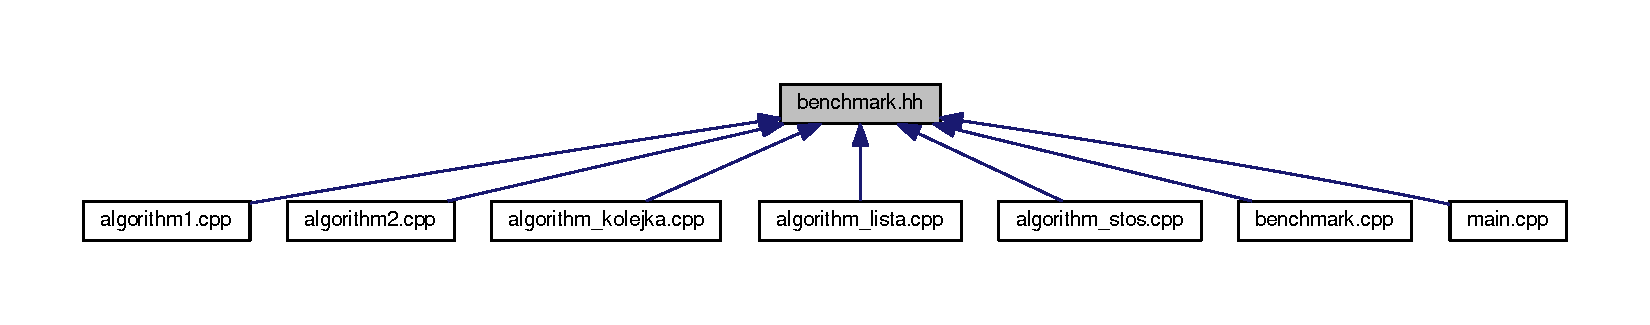
\includegraphics[width=350pt]{benchmark_8hh__dep__incl}
\end{center}
\end{figure}
\subsection*{Classes}
\begin{DoxyCompactItemize}
\item 
class \hyperlink{class_benchmark}{Benchmark}
\begin{DoxyCompactList}\small\item\em Klasa \hyperlink{class_benchmark}{Benchmark} modelujaca program benchmarkujacy. Obiekt tego typu reprezentuje program sprawdzajacy szybkosc wykonywania algorytmow. \end{DoxyCompactList}\end{DoxyCompactItemize}
\subsection*{Macros}
\begin{DoxyCompactItemize}
\item 
\#define \hyperlink{benchmark_8hh_a70ed59adcb4159ac551058053e649640}{S\-I\-Z\-E}~100
\end{DoxyCompactItemize}


\subsection{Macro Definition Documentation}
\hypertarget{benchmark_8hh_a70ed59adcb4159ac551058053e649640}{\index{benchmark.\-hh@{benchmark.\-hh}!S\-I\-Z\-E@{S\-I\-Z\-E}}
\index{S\-I\-Z\-E@{S\-I\-Z\-E}!benchmark.hh@{benchmark.\-hh}}
\subsubsection[{S\-I\-Z\-E}]{\setlength{\rightskip}{0pt plus 5cm}\#define S\-I\-Z\-E~100}}\label{benchmark_8hh_a70ed59adcb4159ac551058053e649640}


Definition at line 4 of file benchmark.\-hh.


\hypertarget{generate_8cpp}{}\section{generate.\+cpp File Reference}
\label{generate_8cpp}\index{generate.\+cpp@{generate.\+cpp}}
{\ttfamily \#include $<$fstream$>$}\\*
{\ttfamily \#include $<$iostream$>$}\\*
{\ttfamily \#include $<$cstdlib$>$}\\*
Include dependency graph for generate.\+cpp\+:\nopagebreak
\begin{figure}[H]
\begin{center}
\leavevmode
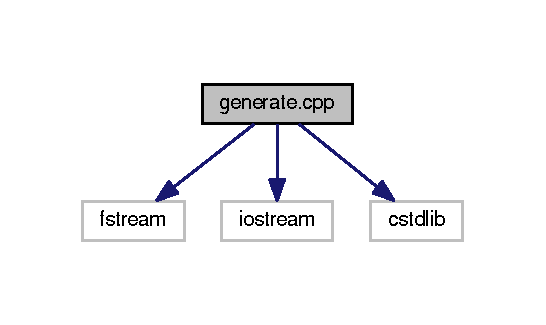
\includegraphics[width=262pt]{generate_8cpp__incl}
\end{center}
\end{figure}
\subsection*{Macros}
\begin{DoxyCompactItemize}
\item 
\#define \hyperlink{generate_8cpp_a70ed59adcb4159ac551058053e649640}{S\+I\+Z\+E}~100000
\end{DoxyCompactItemize}
\subsection*{Functions}
\begin{DoxyCompactItemize}
\item 
int \hyperlink{generate_8cpp_ae66f6b31b5ad750f1fe042a706a4e3d4}{main} ()
\begin{DoxyCompactList}\small\item\em Funkcja generowania pliku z danymi wejsciowymi. Generuje liczby losowe od 1 do 51 i zapisuje je do pliku o nazwie data.\+txt. \end{DoxyCompactList}\end{DoxyCompactItemize}


\subsection{Macro Definition Documentation}
\hypertarget{generate_8cpp_a70ed59adcb4159ac551058053e649640}{}\index{generate.\+cpp@{generate.\+cpp}!S\+I\+Z\+E@{S\+I\+Z\+E}}
\index{S\+I\+Z\+E@{S\+I\+Z\+E}!generate.\+cpp@{generate.\+cpp}}
\subsubsection[{S\+I\+Z\+E}]{\setlength{\rightskip}{0pt plus 5cm}\#define S\+I\+Z\+E~100000}\label{generate_8cpp_a70ed59adcb4159ac551058053e649640}


Definition at line 5 of file generate.\+cpp.



\subsection{Function Documentation}
\hypertarget{generate_8cpp_ae66f6b31b5ad750f1fe042a706a4e3d4}{}\index{generate.\+cpp@{generate.\+cpp}!main@{main}}
\index{main@{main}!generate.\+cpp@{generate.\+cpp}}
\subsubsection[{main}]{\setlength{\rightskip}{0pt plus 5cm}int main (
\begin{DoxyParamCaption}
{}
\end{DoxyParamCaption}
)}\label{generate_8cpp_ae66f6b31b5ad750f1fe042a706a4e3d4}

\begin{DoxyRetVals}{Return values}
{\em 0} & -\/ gdy funkcja zadziala poprawnie. \\
\hline
{\em 1} & -\/ gdy wystapi blad otwarcia pliku do zapisu. \\
\hline
\end{DoxyRetVals}


Definition at line 14 of file generate.\+cpp.


\hypertarget{kolejka_8cpp}{\section{kolejka.\-cpp File Reference}
\label{kolejka_8cpp}\index{kolejka.\-cpp@{kolejka.\-cpp}}
}
{\ttfamily \#include $<$iostream$>$}\\*
{\ttfamily \#include \char`\"{}kolejka.\-hh\char`\"{}}\\*
Include dependency graph for kolejka.\-cpp\-:\nopagebreak
\begin{figure}[H]
\begin{center}
\leavevmode
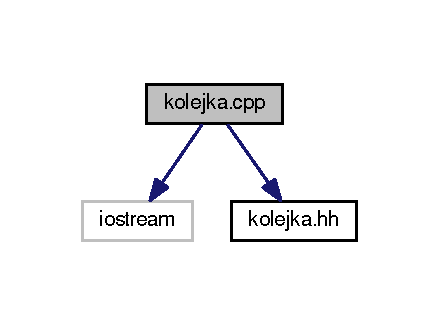
\includegraphics[width=212pt]{kolejka_8cpp__incl}
\end{center}
\end{figure}

\hypertarget{kolejka_8hh}{\section{kolejka.\-hh File Reference}
\label{kolejka_8hh}\index{kolejka.\-hh@{kolejka.\-hh}}
}
This graph shows which files directly or indirectly include this file\-:\nopagebreak
\begin{figure}[H]
\begin{center}
\leavevmode
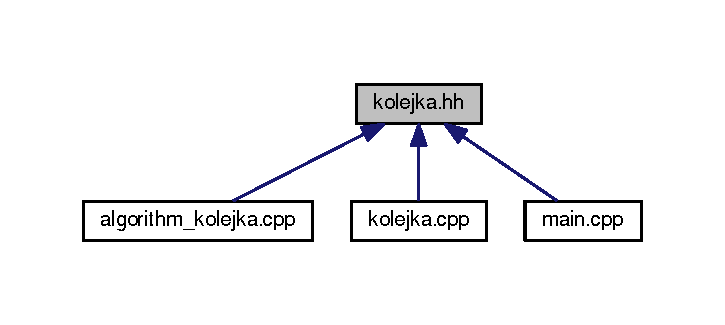
\includegraphics[width=348pt]{kolejka_8hh__dep__incl}
\end{center}
\end{figure}
\subsection*{Classes}
\begin{DoxyCompactItemize}
\item 
class \hyperlink{class_kolejka}{Kolejka}
\begin{DoxyCompactList}\small\item\em Klasa \hyperlink{class_kolejka}{Kolejka} modelujaca strukture danych typu kolejka. Obiekt tego typu reprezentuje strukture danych typu kolejka wraz z operacjami mozliwymi do wykonania na tej strukturze. \end{DoxyCompactList}\end{DoxyCompactItemize}

\hypertarget{lista_8cpp}{\section{lista.\-cpp File Reference}
\label{lista_8cpp}\index{lista.\-cpp@{lista.\-cpp}}
}
{\ttfamily \#include $<$iostream$>$}\\*
{\ttfamily \#include \char`\"{}lista.\-hh\char`\"{}}\\*
Include dependency graph for lista.\-cpp\-:\nopagebreak
\begin{figure}[H]
\begin{center}
\leavevmode
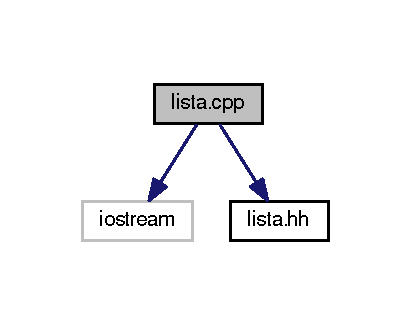
\includegraphics[width=199pt]{lista_8cpp__incl}
\end{center}
\end{figure}

\hypertarget{lista_8hh}{\section{lista.\-hh File Reference}
\label{lista_8hh}\index{lista.\-hh@{lista.\-hh}}
}
This graph shows which files directly or indirectly include this file\-:\nopagebreak
\begin{figure}[H]
\begin{center}
\leavevmode
\includegraphics[width=323pt]{lista_8hh__dep__incl}
\end{center}
\end{figure}
\subsection*{Classes}
\begin{DoxyCompactItemize}
\item 
class \hyperlink{class_lista}{Lista}
\begin{DoxyCompactList}\small\item\em Klasa \hyperlink{class_lista}{Lista} modelujaca strukture danych typu lista. Obiekt tego typu reprezentuje strukture danych typu lista wraz z operacjami mozliwymi do wykonania na tej strukturze. \end{DoxyCompactList}\item 
struct \hyperlink{struct_lista_1_1_komorka}{Lista\-::\-Komorka}
\begin{DoxyCompactList}\small\item\em Struktura \hyperlink{struct_lista_1_1_komorka}{Komorka}. Obiekt tego typu reprezentuje pojedyncza komorke wraz ze wskaznikiem na nastepna komorke listy. \end{DoxyCompactList}\end{DoxyCompactItemize}

\hypertarget{main_8cpp}{}\section{main.\+cpp File Reference}
\label{main_8cpp}\index{main.\+cpp@{main.\+cpp}}
{\ttfamily \#include $<$iostream$>$}\\*
{\ttfamily \#include \char`\"{}benchmark.\+hh\char`\"{}}\\*
{\ttfamily \#include \char`\"{}stos.\+hh\char`\"{}}\\*
{\ttfamily \#include \char`\"{}kolejka.\+hh\char`\"{}}\\*
{\ttfamily \#include \char`\"{}lista.\+hh\char`\"{}}\\*
{\ttfamily \#include \char`\"{}tab\+\_\+lista.\+hh\char`\"{}}\\*
{\ttfamily \#include \char`\"{}algorithm\+\_\+stos.\+hh\char`\"{}}\\*
{\ttfamily \#include \char`\"{}algorithm\+\_\+kolejka.\+hh\char`\"{}}\\*
{\ttfamily \#include \char`\"{}algorithm\+\_\+lista.\+hh\char`\"{}}\\*
{\ttfamily \#include \char`\"{}algorithm2.\+hh\char`\"{}}\\*
Include dependency graph for main.\+cpp\+:\nopagebreak
\begin{figure}[H]
\begin{center}
\leavevmode
\includegraphics[width=350pt]{main_8cpp__incl}
\end{center}
\end{figure}
\subsection*{Functions}
\begin{DoxyCompactItemize}
\item 
int \hyperlink{main_8cpp_ae66f6b31b5ad750f1fe042a706a4e3d4}{main} ()
\begin{DoxyCompactList}\small\item\em Funkcja tworzaca i testujaca algorytm. Wczytuje dane otrzymane na strumien wejsciowy do tablicy data\mbox{[}\mbox{]}. Nastepnie tworzy obiekt \hyperlink{class_benchmark}{Benchmark} oraz obiekt Potegowanie. Pozniej uruchamia metode testujaca w obiekcie klasy \hyperlink{class_benchmark}{Benchmark} dla obiektu klasy Potegowanie. \end{DoxyCompactList}\end{DoxyCompactItemize}


\subsection{Function Documentation}
\hypertarget{main_8cpp_ae66f6b31b5ad750f1fe042a706a4e3d4}{}\index{main.\+cpp@{main.\+cpp}!main@{main}}
\index{main@{main}!main.\+cpp@{main.\+cpp}}
\subsubsection[{main}]{\setlength{\rightskip}{0pt plus 5cm}int main (
\begin{DoxyParamCaption}
{}
\end{DoxyParamCaption}
)}\label{main_8cpp_ae66f6b31b5ad750f1fe042a706a4e3d4}

\begin{DoxyRetVals}{Return values}
{\em 0} & -\/ domyslna wartosc zwracana przez funkcje. \\
\hline
\end{DoxyRetVals}


Definition at line 21 of file main.\+cpp.


\hypertarget{stos_8cpp}{}\section{stos.\+cpp File Reference}
\label{stos_8cpp}\index{stos.\+cpp@{stos.\+cpp}}
{\ttfamily \#include $<$iostream$>$}\\*
{\ttfamily \#include \char`\"{}stos.\+hh\char`\"{}}\\*
Include dependency graph for stos.\+cpp\+:\nopagebreak
\begin{figure}[H]
\begin{center}
\leavevmode
\includegraphics[width=197pt]{stos_8cpp__incl}
\end{center}
\end{figure}

\hypertarget{stos_8hh}{}\section{stos.\+hh File Reference}
\label{stos_8hh}\index{stos.\+hh@{stos.\+hh}}
This graph shows which files directly or indirectly include this file\+:\nopagebreak
\begin{figure}[H]
\begin{center}
\leavevmode
\includegraphics[width=320pt]{stos_8hh__dep__incl}
\end{center}
\end{figure}
\subsection*{Classes}
\begin{DoxyCompactItemize}
\item 
class \hyperlink{class_stos}{Stos}
\begin{DoxyCompactList}\small\item\em Klasa \hyperlink{class_stos}{Stos} modelujaca strukture danych typu stos. Obiekt tego typu reprezentuje strukture danych typu stos wraz z operacjami mozliwymi do wykonania na tej strukturze. \end{DoxyCompactList}\end{DoxyCompactItemize}

\hypertarget{strona-glowna_8dox}{}\section{strona-\/glowna.dox File Reference}
\label{strona-glowna_8dox}\index{strona-\/glowna.\+dox@{strona-\/glowna.\+dox}}

\hypertarget{tab__lista_8cpp}{}\section{tab\+\_\+lista.\+cpp File Reference}
\label{tab__lista_8cpp}\index{tab\+\_\+lista.\+cpp@{tab\+\_\+lista.\+cpp}}
{\ttfamily \#include $<$iostream$>$}\\*
{\ttfamily \#include \char`\"{}tab\+\_\+lista.\+hh\char`\"{}}\\*
Include dependency graph for tab\+\_\+lista.\+cpp\+:\nopagebreak
\begin{figure}[H]
\begin{center}
\leavevmode
\includegraphics[width=215pt]{tab__lista_8cpp__incl}
\end{center}
\end{figure}

\hypertarget{tab__lista_8hh}{\section{tab\-\_\-lista.\-hh File Reference}
\label{tab__lista_8hh}\index{tab\-\_\-lista.\-hh@{tab\-\_\-lista.\-hh}}
}
This graph shows which files directly or indirectly include this file\-:\nopagebreak
\begin{figure}[H]
\begin{center}
\leavevmode
\includegraphics[width=323pt]{tab__lista_8hh__dep__incl}
\end{center}
\end{figure}
\subsection*{Classes}
\begin{DoxyCompactItemize}
\item 
class \hyperlink{class_tab_lista}{Tab\-Lista}
\begin{DoxyCompactList}\small\item\em Klasa \hyperlink{class_tab_lista}{Tab\-Lista} modelujaca strukture danych typu lista. Obiekt tego typu reprezentuje strukture danych typu lista zaimplementowana na tablicy dynamicznej. Obiekt zawiera rowniez podstowe metody listy. \end{DoxyCompactList}\end{DoxyCompactItemize}

%--- End generated contents ---

% Index
\newpage
\phantomsection
\addcontentsline{toc}{chapter}{Index}
\printindex

\end{document}
